\section{Implement Details and Complexity Analysis} \label{sec:complex}

\subsection{Background: Time Variable ODE}

A numerical ODE solver integrates a single ODE system $\frac{d \textbf{x}}{d t}=f(t, \textbf{x})$, where $\textbf{x} \in \mathbb{R}^d$ and $f: \mathbb{R}^{d+1} \rightarrow \mathbb{R}^d$. Given an initial state $\textbf{x}_{t_0}$, the ODE solver produces $\textbf{x}_{t_1}, \textbf{x}_{t_2}, ..., \textbf{x}_{t_N}$, which represents the latent state for each time point~\cite{chen2018neural}, i.e.,
\begin{equation}
    \textbf{x}_{t_1}, \textbf{x}_{t_2}, \ldots, \mathbf{z}_{t_N}=\operatorname{ODESolve}\left(\textbf{x}_{t_0}, f, t_0, \ldots, t_N\right) ~.
\label{eq:ode}
\end{equation}
To obtain the solution of Eq. (\ref{eq:ode}), it requires the ODE solver to integrate over the interval $[t_0, t_N]$.

\paragraph{Varied time intervals} Now, we suppose that we need to solve $M$ dynamic system that has different time intervals. Let denote for the $i$-th system, the start point is $t_0^{(i)}$ and the endpoint is $t_1^{(i)}$ and the ODE system is defined by $\frac{d \textbf{x}}{d t}=f(t, \textbf{x})$. We can construct a dummy variable so that the integral interval always starts from $-1$ and ends at $1$ and perform a change of variables to transform every system to use this dummy variable.

For simplifying purposes, we assume that a single system that integrates from $t_0$ to $t_1$ with $f(t, \textbf{x})$ can control the differential equation and the solution of $\textbf{x}(t)$. We introduce a dummy variable $s=\frac{2t - t_0 - t_1}{t_1 - t_0}$ and a solution $\mathbf{\tilde{x}}(s)$ in a fix interval $[-1, 1]$ satisfies
\begin{equation}
    \tilde{\textbf{x}}(s) = \textbf{x}(\frac{s(t_1 - t_0) + t_0 + t_1}{2}) ~.
\end{equation}
The differential equation that solve $\mathbf{x}$ follows that
\begin{equation}
\begin{aligned}
\tilde{f}(s, \tilde{\textbf{x}}(s)) = \frac{d \tilde{\textbf{x}}(s)}{d s} & =\left.\frac{d \textbf{x}(t)}{d t}\right|_{t=\frac{s(t_1 - t_0) + t_0 + t_1}{2}} \frac{d t}{d s} \\
& =\left.f(t, \textbf{x}(t))\right|_{t=\frac{s(t_1 - t_0) + t_0 + t_1}{2}}\left(\frac{t_1 - t_0}{2}\right) \\
& =f\left(\frac{s(t_1 - t_0) + t_0 + t_1}{2}, \tilde{\textbf{x}}(s)\right)\left(\frac{t_1 - t_0}{2}\right) ~.
\end{aligned}
\end{equation}
Since $\tilde{\textbf{x}}(-1)=\textbf{x}(t_0)$ and $\tilde{\textbf{x}}(1)=x_{t_1}$, thus we have
\begin{equation}
    \textbf{x}(t_1)= \operatorname{ODESolve}(\textbf{x}(t_0), f, t_0, t_1) = \operatorname{ODESolve}(\tilde{\textbf{x}}(-1), \tilde{f}, -1, 1) ~.
\end{equation}

\subsection{Background: Approximating Definite Integral of a Function} \label{sec:approximating}

Given a function $f$ that integrates over an interval $[-1, 1]$, a simple method to approximate it is to assume that the change is linear over time, i.e.,
\begin{equation}
\int_{-1}^{1} f(x) d x \approx \frac{f(-1) + f(1)}{2} ~.
\end{equation}
Besides, in numerical analysis, Gauss–Legendre Quadrature provides a more accurate way to approximate an integral over an interval $[-1, 1]$, i.e.,
\begin{equation}
\int_{-1}^1 f(x) \mathrm{d} x \approx \sum_j \omega_j f\left(\xi_j\right) ~,
\end{equation}
where $\left\{\omega_j\right\}$ and $\left\{\xi_j\right\}$ are quadrature weights and nodes such that $-1 \leq \xi_1 < ... < \xi_k \leq 1$.

\subsection{Putting it all together}

Given an irregular-sampled sequence, $\Gamma=[ (x_1, t_1), (x_2, t_2), ..., (x_N, t_N)]$, where $x_i \in \mathbb{R}^{d}$ is the input feature of the $i$-th tokens happen at time $t_i$ and $N$ is the length of the sequence. We analyze the time and space complexity for an autoregressive task where the output of each observation is required for a particular classification or regression task. Specifically, for Eq. (\ref{eq:attn}), $\boldsymbol{\mathrm{\alpha}}_i(t_1), \boldsymbol{\mathrm{\alpha}}_i(t_2), \ldots, \boldsymbol{\mathrm{\alpha}}_i(t_N)$ is required to form the output of Transformer. Therefore, the key difficulty is to solve Eq. (\ref{eq:attn}). By using the numerical approximation method, we have
\begin{equation}
    \boldsymbol{\mathrm{\alpha}}_i(t_j) = \frac{\int_{t_i}^{t_j} \boldsymbol{\mathrm{q}}(\tau) \cdot \boldsymbol{\mathrm{k}}_i(\tau)^\top \text{d}\tau}{t_j - t_i} = \frac{1}{2} \int_{-1}^{1} \tilde{\boldsymbol{\mathrm{q}}}_{i,j}(\tau) \cdot \tilde{\boldsymbol{\mathrm{k}}}_{i,j}(\tau)^\top \text{d} \tau \approx  \frac{1}{2} \sum_{p=1}^{P} \gamma_p \tilde{\boldsymbol{\mathrm{q}}}_{i,j}(\xi_p) \cdot \tilde{\boldsymbol{\mathrm{k}}}_{i,j}(\xi_p)^{\top} ~,
\end{equation}
where $\tilde{\boldsymbol{\mathrm{q}}}_{i,j}$ and $\tilde{\boldsymbol{\mathrm{k}}}_{i,j}$ follows that:
\begin{equation}
\begin{aligned}
  \tilde{\boldsymbol{\mathrm{q}}}_{i,j}(s) & = \boldsymbol{\mathrm{q}}\left(\frac{s(t_i - t_j) + t_i + t_j}{2}\right) ~,  \\
  \tilde{\boldsymbol{\mathrm{k}}}_{i,j}(s) & = \boldsymbol{\mathrm{q}}_j\left(\frac{s(t_i - t_j) + t_i + t_j}{2}\right) ~.
\end{aligned}
\end{equation}
We use $\hat{\boldsymbol{\mathrm{k}}}_{i,j}$ to denote $\frac{d \tilde{\boldsymbol{\mathrm{k}}}_{i,j}(s)}{d s}$. Thus, $\boldsymbol{\mathrm{\alpha}}_i(t_j)$ can be solved by paralleling $N^2$ ODE solvers. Specifically, $\tilde{\boldsymbol{\mathrm{k}}}_{i,j}(\xi_p)$ is given by
\begin{equation}
    \tilde{\boldsymbol{\mathrm{k}}}_{i,j}(\xi_1), \tilde{\boldsymbol{\mathrm{k}}}_{i,j}(\xi_2), ..., \tilde{\boldsymbol{\mathrm{k}}}_{i,j}(\xi_p) = \operatorname{ODESolver} (\boldsymbol{\mathrm{k}}_j(t_j), \hat{\boldsymbol{\mathrm{k}}}_{i,j}, -1, \xi_1, \xi_2, ..., \xi_p) ~.
\end{equation}

As for $\tilde{\boldsymbol{\mathrm{q}}}_{i,j}(\xi_k)$, since the input sequence is irregularly sampled and discrete in time, we propose to use interpolation methods~\cite{kidger2020neural} (e.g., linear interpolation or cubic interpolation) method on $Q$ to construct a continuous-time query. Therefore $\tilde{\boldsymbol{\mathrm{q}}}_{i,j}(\xi_k)$ can be easily calculated in $O(d)$ time complexity.


\section{Representation Power of ContiFormer} \label{sec:proof}

In the section, we mathematically prove that by curated designs of function hypothesis, many Transformer variants can be covered as a special case of ContiFormer. For simplification, we only discuss the self-attention mechanism, where $Q, K, V \in \mathbb{R}^{N \times d}$.

\subsection{Transformer Variants} \label{sec:variants}

We first show several Transformer-based methods for irregular time series. Most of these methods shown below calculate $N \times N$ attention matrix and multiply it with $V$\footnote{Throughout the proof section, we define $\boldsymbol{\mathrm{v}}_i(t_i)=\boldsymbol{\mathrm{v}}_i(t_i)=V_i$, and focus on the proof of attention matrix.}. 

\paragraph{Vanilla Transformer}

Given query $Q \in \mathbb{R}^{N \times d}$ and $V \in \mathbb{R}^{N \times d}$, the attention matrix of a vanilla transformer~\cite{vaswani2017attention} is calculated as 
\begin{equation}
\operatorname{Attn}(Q, K)=\left[\begin{array}{cccc}
Q_1 \cdot K_1^\top & Q_1 \cdot K_2^\top & \cdots & Q_1 \cdot K_N^\top \\
Q_2 \cdot K_1^\top & Q_2 \cdot K_2^\top & \cdots & Q_2 \cdot K_N^\top \\
\vdots & \vdots & \ddots & \vdots \\
Q_N \cdot K_1^\top & Q_N \cdot K_2^\top & \cdots & Q_N \cdot K_N^\top
\end{array}\right] ~,
\end{equation}
and the output of the self-attention mechanism is obtained by\footnote{For simplification, we assume single-head attention is adopted throughout the proof.}
\begin{equation}
Z_i = \operatorname{Softmax}(\operatorname{Attn}(Q, K)_i) V ~.
\end{equation}

\paragraph{Kernelized Attention}

Kernelized attention mechanism \footnote{Not to be confused with methods that regard kernels as a form of approximation of the attention matrix.} incorporate time information through defining specific kernel function $k(x, x')$ and replace the attention matrix with
\begin{equation}
\operatorname{Attn}(Q, K)=\left[\begin{array}{cccc}
Q_1 \cdot K_1^\top * k(t_1, t_1) & Q_1 \cdot K_2^\top * k(t_1, t_2) & \cdots & Q_1 \cdot K_N^\top * k(t_1, t_N) \\
Q_2 \cdot K_1^\top * k(t_2, t_1) & Q_2 \cdot K_2^\top * k(t_2, t_2) & \cdots & Q_2 \cdot K_N^\top * k(t_2, t_N) \\
\vdots & \vdots & \ddots & \vdots \\
Q_N \cdot K_1^\top * k(t_N, t_1) & Q_N \cdot K_2^\top * k(t_N, t_2) & \cdots & Q_N \cdot K_N^\top * k(t_N, t_N)
\end{array}\right] ~.
\end{equation}
Kernel functions are typically symmetric and hold that $\phi(x, x)=1$ for any $x$. For instance, NSTKA~\cite{ma2022non} propose a learnable Generalized Spectral Mixture (GSM) kernel, i.e.,
\begin{equation}
\begin{aligned}
k_\text{GSM}\left(x, x'\right) &=
 \sum_i \phi_i(x) \phi_i\left(x'\right) k_{\text{Gibbs}, i}\left(x, x'\right) \cos \left(2 \pi\left(\mu_i(x) x-\mu_i\left(x'\right) x'\right)\right) ~, \\
\text{ where } k_{\text{Gibbs}, i}\left(x, x'\right) &= \sqrt{\frac{2 l_i(x) l_i\left(x'\right)}{l_i(x)^2+l_i\left(x'\right)^2}} \exp \left(-\frac{\left(x-x'\right)^2}{l_i(x)^2+l_i\left(x'\right)^2}\right) .
\end{aligned}
\end{equation}
where $\mu_i(x)$ denotes the mean, lengthscale as $l_i(x)$ and input-dependent weight as $\phi_i(x)$. 

\paragraph{Time Embedding Methods}

Time embedding methods learn a time representation, adding or concatenating it with the input embedding, i.e.,
\begin{equation}
\operatorname{\widehat{Attn}}(Q, K)=\left[\begin{array}{cccc}
(Q_1, \Phi(t_1)) \cdot (K_1, \Phi(t_1))^\top & \cdots & (Q_1, \Phi(t_1)) \cdot (K_N, \Phi(t_N))^\top  \\ 
(Q_2, \Phi(t_2)) \cdot (K_1, \Phi(t_1))^\top  & \cdots & (Q_2, \Phi(t_2)) \cdot (K_N, \Phi(t_N))^\top \\ 
\vdots & \ddots & \vdots \\
(Q_N, \Phi(t_N)) \cdot (K_1, \Phi(t_1))^\top & \cdots & (Q_N, \Phi(t_N)) \cdot (K_N, \Phi(t_N))^\top
\end{array}\right] ~,
\end{equation}
where $(\cdot, \cdot)$ is the concatenation of two vectors, $\Phi(\cdot): \mathbb{R} \rightarrow \mathbb{R}^{d}$ is a learnable time representation. For simplification, we assume that time embedding is concatenated with the input embedding and ignore linear transformation on the time embedding.\footnote{Using the concatenation operation, we have $(Q_i, \Phi(t_i)) \cdot (K_j, \Phi(t_j))^\top=Q_i \cdot K_j^\top + \Phi(t_i) \cdot \Phi(t_j)^\top$.} 

For instance, Mercer~\cite{xu2019self} transforms the periodic kernel function into the high-dimensional space spanned by truncated Fourier basis under certain frequencies ($\{\omega_i\}$) and coefficients $\{c_i\}$, i.e.,
\begin{equation}
\begin{aligned}
\Phi(t) \mapsto \Phi_d^{\mathcal{M}} & =\left[\Phi_{\omega_1, d}^{\mathcal{M}}(t), \ldots, \Phi_{\omega_k, d}^{\mathcal{M}}(t)\right]^{\top} ~,\\
\text{ where } \Phi_\omega^{\mathcal{M}}(t) & =\left[\sqrt{c_1}, \ldots, \sqrt{c_{2 j}} \cos \left(\frac{j \pi t}{\omega}\right), \sqrt{c_{2 j+1}} \sin \left(\frac{j \pi t}{\omega}\right), \ldots\right] ~.
\end{aligned}
\end{equation}
mTAN~\cite{shukla2021multi} generalizes the notion of a positional encoding used in Transformer-based models to continuous-time domain, i.e., 
\begin{equation}
\Phi(t) = \phi(t) \cdot \textbf{w} ~,
\end{equation}
where $\textbf{w} \in \mathbb{R}^{d \times d}$ is a linear transformation \footnote{In the original paper, the equation is defined as $\Phi(t_i, t_j) = \phi(t_i) \textbf{w}\textbf{v}^\top \phi(t_j)$. For simplicity purpose, we assume that $\textbf{w} = \textbf{v}$.} and 
\begin{equation}
\phi(t)_i = \begin{cases}
    \omega_0 \cdot t + \phi_0, & \text{if } i = 0\\
    \sin (\omega_i \cdot t + \phi_i), & \text{if } 0 < i \leq d
    \end{cases} ~,
\end{equation}
where $\omega$ and $\phi$ are learnable weights. Furthermore, mTAN assumes that $Q=K=\textbf{0}$.

Besides, since $\operatorname{Softmax}(\textbf{x} + c)=\operatorname{Softmax}(\textbf{x})$, where $\textbf{x}$ is a vector and $c$ is a constant. The following equation holds,
\begin{equation}
\operatorname{Softmax}(\operatorname{Attn}(Q, K)) = \operatorname{Softmax}(\operatorname{\widehat{Attn}}(Q, K)) ~,
\end{equation}
where the matrix form of $\operatorname{Softmax}$ normalize each row of the matrix and 
\begin{equation}
\begin{aligned}
\operatorname{Attn}& (Q, K)= \\
& \left[\begin{array}{cccc}
Q_1 \cdot K_1^\top & \cdots & Q_1 \cdot K_N + \Phi(t_1) \cdot (\Phi(t_N) - \Phi(t_1))^\top  \\ 
Q_2 \cdot K_1 + \Phi(t_2) \cdot (\Phi(t_2) - \Phi(t_1))^\top  & \cdots & Q_2 \cdot K_N + \Phi(t_2) \cdot (\Phi(t_N) - \Phi(t_2))^\top \\ 
\vdots & \ddots & \vdots \\
Q_N \cdot K_1 + \Phi(t_N) \cdot (\Phi(t_1) - \Phi(t_N))^\top & \cdots & Q_N \cdot K_N^\top
\end{array}\right] ~.
\end{aligned}
\end{equation}

\subsection{Proof of Extension and Universal Approximation} 

\begin{lemma}[Existence of Continuously Differentiable Vector Function] 
Given a continuously differentiable vector function $u: \mathbb{R} \rightarrow \mathbb{R}^d \in \mathcal{C}^1$, such that $\forall x \in \mathbb{R}, \|u(x)\|_2 < \infty, \|u(x)\|_0 = d$ and a continuously differentiable function $w: \mathbb{R} \rightarrow \mathbb{R} \in \mathcal{C}^1$, there always exists another continuously differentiable vector function $v: \mathbb{R} \rightarrow \mathbb{R}^d \in \mathcal{C}^1$ with a fixed point $p$ satisfying $u(p) \cdot v(p)^\top = w(p)$, such that $\forall x \in \mathbb{R}, u(x) \cdot v(x)^\top = w(x)$ holds. \footnote{Consider an open set $\mathcal{U}$ on the real line and a function $f$ defined on $\mathcal{U}$ with real values. Let $k$ be a non-negative integer. The function $f$ is said to be of differentiability class $\mathcal{C}^{k}$ if the derivatives  $f',f'',\dots ,f^{(k)}$ exist and are continuous on $\mathcal{U}$.}
\end{lemma}

\begin{proof}
Throughout the proof, we define $\xi := v(p)$.

Since $\forall x \in \mathbb{R}, 0 <\|u(x)\|_2 < \infty$, we define
\begin{equation}
v(x) = \frac{u(x)}{\|u(x)\|_2^2} \cdot w(x) + k(x) ~,
\end{equation}
where $k(x) \in \mathcal{C}^1$ such that $\forall x \in \mathbb{R}, u(x) \cdot k(x)^\top=0$ holds. Therefore, for $\forall x  \in \mathbb{R}$, we have
\begin{equation}
u(x) \cdot v(x)^\top = u(x) \cdot \left( \frac{u(x)}{\|u(x)\|_2^2} \cdot w(x) + k(x) \right) = w(x) + u(x) \cdot k(x) = w(x) ~.
\end{equation}
Thus, we only need to prove the existence of $k(x)$. Since $v(x)$ has a fixed point at $p$, therefore,
\begin{equation}
k(p) = \xi - \frac{u(p)}{\|u(p)\|_2^2} \cdot w(p) ~.
\label{eq:cons}
\end{equation}
Let $z[i]$ denote the $i$-th element of a vector $z$, thus, Eq. (\ref{eq:cons}) is equivalent to
\begin{equation}
k(p)[i] = \xi[i] - \frac{u(p)[i]}{\|u(p)\|_2^2} * w(p)[i] ~,
\end{equation}
for $i \in [1, d]$. Since we have $u(p) \cdot v(p)^\top = w(p)$, thus,
\begin{equation}
k(p) \cdot u(p)^\top = \xi \cdot u(p)^\top - w(p) = 0 ~.
\label{eq:kf}
\end{equation}

We denote $c_i := k(p)[i] * u(p)[i]$. Since Eq. (\ref{eq:kf}) holds, therefore $\sum_{i=1}^{d} c_i=0$. Finally, we can construct $k(x)$ as
\begin{equation}
k(x) = \left[\begin{array}{cccc}
k(x)[1]  \\ 
k(x)[2] \\ 
\vdots  \\
k(x)[d] \end{array}\right]^\top = \left[\begin{array}{cccc}
c_1 / u(x)[1]  \\ 
c_2 / u(x)[2] \\ 
\vdots  \\
c_d / u(x)[d] \end{array}\right]^\top ~.
\end{equation}
Since $u, w \in \mathcal{C}^1$, therefore $k \in \mathcal{C}^1$, thus $v \in \mathcal{C}^1$.
\end{proof}


\begin{lemma}[Existence of $\boldsymbol{k}_i(t)$]
Given a continuously differentiable vector function $\boldsymbol{\mathrm{q}}: \mathbb{R} \rightarrow \mathbb{R}^d \in \mathcal{C}^1$ such that $\forall x \in \mathbb{R}, \|\boldsymbol{\mathrm{q}}(x)\|_2 < \infty, \|\boldsymbol{\mathrm{q}}(x)\|_0 = d$ and a continuously differentiable function $f: \mathbb{R} \rightarrow \mathbb{R} \in \mathcal{C}^2$ and a vector $K_i \in \mathbb{R}^{d}$ and satisfies $f(t_i) = \boldsymbol{\mathrm{q}}(t_i) \cdot K_i^\top$, there always exist a continuously differentiable vector function $\boldsymbol{\mathrm{k}}_i: \mathbb{R} \rightarrow \mathbb{R}^d$, such that the following statements hold:
\begin{itemize}[leftmargin=5mm]
    \item $\boldsymbol{\mathrm{k}}_i(t_i)=K_i$,
    \item $\forall t \in \mathbb{R}, t \neq t_i, \boldsymbol{\mathrm{\alpha}}_i(t) := \frac{\int_{t_i}^t \boldsymbol{\mathrm{q}}(\tau) \cdot \boldsymbol{\mathrm{k}}_i(\tau)^\top \text{d} \tau}{t-t_i} = f(t)$.
\end{itemize}
\end{lemma}

\begin{proof}
Since $t \neq t_i$, we have
\begin{equation}
\begin{gathered}
\begin{aligned}
& \boldsymbol{\mathrm{\alpha}}_i(t) = f(t) \\
 \iff & \boldsymbol{\mathrm{\alpha}}_i(t) (t - t_i) = f(t) (t - t_i) \\
 \stackrel{\textcircled{\tiny{1}}}{\iff} & \frac{\text{d} \boldsymbol{\mathrm{\alpha}}_i(t) (t - t_i)}{\text{d} t} = \frac{\text{d} f(t) (t - t_i)}{\text{d} t} \\ 
 \iff & \boldsymbol{\mathrm{q}}(t) \cdot  \boldsymbol{\mathrm{k}}_i(t)^\top = \frac{\text{d} f}{\text{d} t}(t - t_i) + f(t) ~, \\
\end{aligned}
\end{gathered}
\label{eq:pp}
\end{equation}
where $\textcircled{\tiny{1}}$ holds since we can define $\boldsymbol{\mathrm{\alpha}}_i(t_i)=f(t_i)$. Besides, since
\begin{equation}
\lim_{|\epsilon| \rightarrow 0} \boldsymbol{\mathrm{\alpha}}_i(t_i + \epsilon) = \lim_{|\epsilon| \rightarrow 0} \frac{\int_{t_i}^{t_i + \epsilon} \boldsymbol{\mathrm{q}}(\tau) \cdot \boldsymbol{\mathrm{k}}_i(\tau) \text{d} \tau}{\epsilon} = \boldsymbol{\mathrm{q}}(t_i) \cdot \boldsymbol{\mathrm{k}}_i(t_i)^\top = \boldsymbol{\mathrm{q}}(t_i) \cdot K_i^\top ~,
\end{equation}
such a definition does not break the continuity of $\boldsymbol{\mathrm{\alpha}}$.

Since $f \in \mathcal{C}^2$, therefore we denote $g(t) := \frac{\text{d} f}{\text{d} t}(t - t_i) + f(t) \in \mathcal{C}^1$. Besides, 
\begin{equation}
g(t_i) = f(t_i) = \boldsymbol{\mathrm{q}}(t_i)\cdot K_i^\top   =  \boldsymbol{\mathrm{q}}(t_i) \cdot \boldsymbol{\mathrm{k}}_i(t_i)^\top 
\end{equation}

By using \textbf{Lemma 1} with $g$ corresponding to $w$, $\boldsymbol{\mathrm{q}}$ to $u$, $\boldsymbol{\mathrm{k}}_i$ to $v$ and $p=t_i$, we can prove the existence of $\boldsymbol{\mathrm{k}}_i$ that satisfies Eq. (\ref{eq:pp}).
\end{proof}

\begin{theorem}[Universal Attention Approximation Theorem]
Given query ($Q$) and key ($K$), such that $\|Q_i\|_2 < \infty, \|Q_i\|_0 = d$ for $i \in [1, ..., N]$.
For any attention matrix with formulation defined in Appendix \ref{sec:variants}, i.e., $\operatorname{Attn}(Q, K)$, there always exists a family of continuously differentiable vector functions $k_1(\cdot), k_2(\cdot), \ldots, k_N(\cdot)$, such that the discrete formulation of $[\boldsymbol{\mathrm{\alpha}}_1(\cdot), \boldsymbol{\mathrm{\alpha}}_2(\cdot), ..., \boldsymbol{\mathrm{\alpha}}_N(\cdot)]$ defined by
\begin{equation}
\operatorname{\widetilde{Attn}}(Q, K)=\left[\begin{array}{cccc}
\boldsymbol{\mathrm{\alpha}}_1(t_1) & \boldsymbol{\mathrm{\alpha}}_2(t_1) & \cdots & \boldsymbol{\mathrm{\alpha}}_N(t_1) \\
\boldsymbol{\mathrm{\alpha}}_1(t_2) & \boldsymbol{\mathrm{\alpha}}_2(t_2) & \cdots & \boldsymbol{\mathrm{\alpha}}_N(t_2) \\
\vdots & \vdots & \ddots & \vdots \\
\boldsymbol{\mathrm{\alpha}}_1(t_N) & \boldsymbol{\mathrm{\alpha}}_2(t_N) & \cdots & \boldsymbol{\mathrm{\alpha}}_N(t_N)
\end{array}\right] ~,
\label{eq:proof}
\end{equation}
satisfies that $\operatorname{\widetilde{Attn}}(Q, K) = \operatorname{Attn}(Q, K)$, where 
\begin{equation}
\boldsymbol{\mathrm{\alpha}}_i(t) = 
\frac{\int_{t_i}^t \boldsymbol{\mathrm{q}}(\tau) \cdot \boldsymbol{\mathrm{k}}_i(\tau)^\top \text{d} \tau}{t-t_i} ,  \text{if } t \neq t_i ~,
\end{equation} 
and $\boldsymbol{\mathrm{\alpha}}_i(t_i) = \boldsymbol{\mathrm{q}}(t_i) \cdot \boldsymbol{\mathrm{k}}_i(t_i)^\top$, $\boldsymbol{\mathrm{q}}(t)$ satisfies $\boldsymbol{\mathrm{q}}(t_i)=Q_i$.
\end{theorem}

\begin{proof}
First, we show that the diagonal elements in Eq. (\ref{eq:proof}), i.e., 
\begin{equation}
    \boldsymbol{\mathrm{\alpha}}_i(t_i) = \boldsymbol{\mathrm{q}}(t_i) \cdot \boldsymbol{\mathrm{k}}_i(t_i)^\top = Q_i \cdot K_i^\top ~,
\end{equation}
holds for different forms of attention matrix defined in Appendix \ref{sec:variants}.

Next, for a given $i \in [1, N]$, there exists a continuous cubic spline $h_i: \mathbb{R} \rightarrow \mathbb{R}$ satisfies $h_i(t_j)=\operatorname{Attn}(Q, K)_{j, i}$ for $\forall j \in [1, \ldots, N]$ and $h_i \in \mathcal{C}^2$. By using \textbf{Lemma 2} with $h_i$ corresponding to $f$, there exists a function $\boldsymbol{\mathrm{k}}_i$ such that $\boldsymbol{\mathrm{\alpha}}_i(t) = h_i(t)$. Therefore, $\boldsymbol{\mathrm{\alpha}}_i(t_j) = h_i(t_j)$ for $j \in [1, ..., N]$, and we finish the proof.
\end{proof}

\section{Experiment Details}

\subsection{Modeling Continuous-Time Function} \label{sec:interpolate}

\subsubsection{Background: 2D Spiral}

A spiral is a curve that starts from a central point and gradually moves away from it while turning around it. We consider two types of spirals that start from time $s$ and end at time $e$. The first type of spiral is defined as
\begin{equation}
    \begin{aligned}
        x(t) & = (a + bt) \cdot cos(t) ~,\\
        y(t) & = (a + bt) \cdot sin(t) ~,
    \end{aligned}
\end{equation}
while the second type of spiral is defined as
\begin{equation}
    \begin{aligned}
        x(t) & = \left(a + 50b / \left(e-t\right)\right) \cdot cos(e-t) ~,\\
        y(t) & = \left(a + 50b / \left(e-t\right)\right) \cdot sin(e-t) ~,\\
    \end{aligned}
\end{equation}
where $a$ and $b$ are parameters of the Archimedean spiral.

\subsubsection{Experiment Setting}

We generate 300 spirals and 200/100 spirals are used for training/testing respectively. For each spiral, it randomly belongs to either a clockwise spiral or a counter-clockwise spiral, we sample $a \sim \mathcal{N}(0, \alpha), b \sim \mathcal{N}(0.3, \alpha)$ and we set $\alpha=0.02$ for Table ~\ref{tab:interp}. Also, we add Gaussian noise from $\mathcal{N}(0, \beta)$ to all training samples and we set $\beta=0.1$. We test different models for interpolation and extrapolation. Specifically, each spiral is sampled at 150 equally-spaced time points. To generate an irregular time series, we randomly sample 30 points from the first half of the trajectory. Thus, the first half of the trajectories are used for the interpolation task while the second half of the trajectories, which is totally unobserved during both training and testing, are used for the extrapolation task. All the models are trained for 5000 iterations with a batch size equal to 64.

\subsubsection{Baseline Implementation}

We compare ContiFormer with Neural ODE-based models and Transformer. 

\begin{itemize}[leftmargin=5mm]
    \item \textit{Neural ODE\cite{chen2018neural}.} This model uses the hidden vectors from the last observation as input, and obtain both the interpolation and extrapolation result from a single ODE solver. We train the model by minimizing the mean square loss.
    \item \textit{Latent ODE (w/ RNN Enc)\cite{chen2018neural}.} We run an RNN encoder through the time series and infer the parameters for a posterior over $z_{t_0}$. Next, we sample $\mathbf{z}_{t_0} \sim q\left(\mathbf{z}_{t_0} \mid\left\{\mathbf{x}_{t_i}, t_i\right\}\right)$. Finally, we obtain both the interpolation and extrapolation result from a single ODE solver, i.e., $\operatorname{ODESolve}(\mathbf{z}_{t_0}, f, \theta_f , t_0, . . . , t_M)$, where $(t_0, t_1, ..., t_M)$ is the time of the trajectory. We train the model by maximizing the evidence lower bound (ELBO). 
    \item \textit{Latent ODE (w/ ODE Enc)\cite{rubanova2019latent}.} We replace the RNN encoder in Latent ODE (w/ RNN Enc) with the ODE-RNN encoder following \cite{rubanova2019latent}. Again, we train the model by maximizing the evidence lower bound (ELBO).
    \item \textit{Neural CDE\cite{park2022neural}.} We follow the official implementation to construct the CDE function. For the interpolation, the hidden vectors are directly obtained from the continuous-time path from Neural CDE. For the extrapolation, we input the hidden vectors from the last timestamp of the Neural CDE to a single ODE solver. We train the model by minimizing the mean square loss.
    \item \textit{Transformer\cite{vaswani2017attention}.} In order to obtain the prediction for both seen and unseen time points, we use a learnable mask for unseen inputs. Instead of using position embedding, the input is added with a temporal encoding before forwarding it to the transformer layer. We train the model by minimizing the mean square loss.
    \item \textit{ContiFormer.} We use linear interpolation to deal with unseen observations to avoid the numerical error caused by constructing the continuous-time query. Similar to Transformer, temporal encoding is adopted and the model is trained by minimizing the mean square loss.
\end{itemize}

\begin{table*}[]
    \centering
    \caption{More experimental results on spiral 2d.}
    \resizebox{\textwidth}{!}{%
    \begin{tabular}{c|c|cccccc}
    \toprule
        \multirow{2}{*}{$\alpha$} & \multirow{2}{*}{Metric} & \multirow{2}{*}{Transformer\cite{vaswani2017attention}} & \multirow{2}{*}{Neural ODE\cite{chen2018neural}} & Latent ODE\cite{chen2018neural} & Latent ODE\cite{rubanova2019latent} & \multirow{2}{*}{Neural CDE\cite{park2022neural}} & \multirow{2}{*}{\textbf{ContiFormer}} \\
        & & & & (w/ RNN Enc) & (w/ ODE Enc) & & \\
    \midrule
    \midrule
    \multicolumn{8}{c}{Task = \textit{Interpolation} ($\times 10^{-2}$)} \\
    \midrule
        \multirow{2}{*}{0.02} & RMSE ($\downarrow$) & 1.37 $\pm$ 0.15 & 1.90 $\pm$ 0.17 & 2.09 $\pm$ 0.22 & 4.53 $\pm$ 1.34 & 4.80 $\pm$ 0.50 &  \textbf{0.50 $\pm$ 0.06} \\
        & MAE ($\downarrow$) & 1.42 $\pm$ 0.14 & 1.90 $\pm$ 0.17 & 1.95 $\pm$ 0.26 & 4.25 $\pm$ 1.48 & 5.12 $\pm$ 0.47 & \textbf{0.53 $\pm$ 0.07} \\
    \midrule
        \multirow{2}{*}{0.2} & RMSE ($\downarrow$) & 2.30 $\pm$ 0.51 & 1.88 $\pm$ 0.09 & 3.34 $\pm$ 0.10 & 4.82 $\pm$ 1.97 & 4.60 $\pm$ 1.08 & \textbf{0.42 $\pm$ 0.04} \\
        & MAE ($\downarrow$) & 1.75 $\pm$ 0.18 & 1.58 $\pm$ 0.12 & 3.16 $\pm$ 0.43 & 4.73 $\pm$ 1.21 & 4.58 $\pm$ 0.93 & \textbf{0.42 $\pm$ 0.01} \\
    \midrule
        \multirow{2}{*}{2} & RMSE ($\downarrow$) & 3.75 $\pm$ 0.50 & 2.1 $\pm$ 0.21 & 3.04 $\pm$ 0.48 & 4.49 $\pm$ 1.26 & 2.92 $\pm$ 0.32 & \textbf{0.45 $\pm$ 0.11} \\
        & MAE ($\downarrow$) & 2.33 $\pm$ 0.60 & 2.49 $\pm$ 0.30 & 2.88 $\pm$ 0.54 & 4.12 $\pm$ 1.00 & 2.96 $\pm$ 0.23 & \textbf{0.41 $\pm$ 0.07} \\
    \midrule
    \midrule
    \multicolumn{8}{c}{Task = \textit{Extrapolation} ($\times 10^{-2}$)} \\
    \midrule
    \multirow{2}{*}{0.02} & RMSE ($\downarrow$) & 1.37 $\pm$ 0.11 & 2.07 $\pm$ 0.02 & 1.59 $\pm$ 0.05 & 2.69 $\pm$ 0.82 & 2.24 $\pm$ 0.03 & \textbf{0.64 $\pm$ 0.10} \\
        & MAE ($\downarrow$) & 1.49 $\pm$ 0.12 & 2.02 $\pm$ 0.07 & 1.52 $\pm$ 0.09 & 2.83 $\pm$ 0.88 & 2.38 $\pm$ 0.04 & \textbf{0.65 $\pm$ 0.08} \\
    \midrule
        \multirow{2}{*}{0.2} & RMSE ($\downarrow$) & 2.96 $\pm$ 1.46 & 4.38 $\pm$ 0.35 & 4.78 $\pm$ 0.15 & 5.03 $\pm$ 1.96 & 3.81 $\pm$ 1.02 & \textbf{0.74 $\pm$ 0.10} \\
        & MAE ($\downarrow$) & 2.79 $\pm$ 1.11 & 3.35 $\pm$ 0.43 & 4.02 $\pm$ 0.59 & 4.72 $\pm$ 1.96 & 3.37 $\pm$ 0.78 & \textbf{0.69 $\pm$ 0.09} \\
    \midrule
        \multirow{2}{*}{2} & RMSE ($\downarrow$) & 5.36 $\pm$ 0.97 & 6.02 $\pm$ 0.58 & 5.70 $\pm$ 0.57 & 4.68 $\pm$ 1.70 & 3.44 $\pm$ 1.06 & \textbf{0.75 $\pm$ 0.07} \\
        & MAE ($\downarrow$) & 4.48 $\pm$ 0.82 & 4.84 $\pm$ 0.43 & 4.46 $\pm$ 0.60 & 4.29 $\pm$ 1.34 & 3.32 $\pm$ 0.85 & \textbf{0.69 $\pm$ 0.07} \\
    \bottomrule
    \end{tabular}}
    \label{tab:int2}
\end{table*}

\subsubsection{Experimental Results with Different $\alpha$}

In this subsection, we test Transformer, Neural ODE and ContiFormer with different $\alpha$ to show the robustness of these models. As shown in Table \ref{tab:int2}, our model can achieve the best result on different parameters.

\subsubsection{More Visualization Results}

More visual results with $\alpha$=0.02 can be found in Figure ~\ref{fig:int2}.

\begin{figure}[htbp]
    \centering
    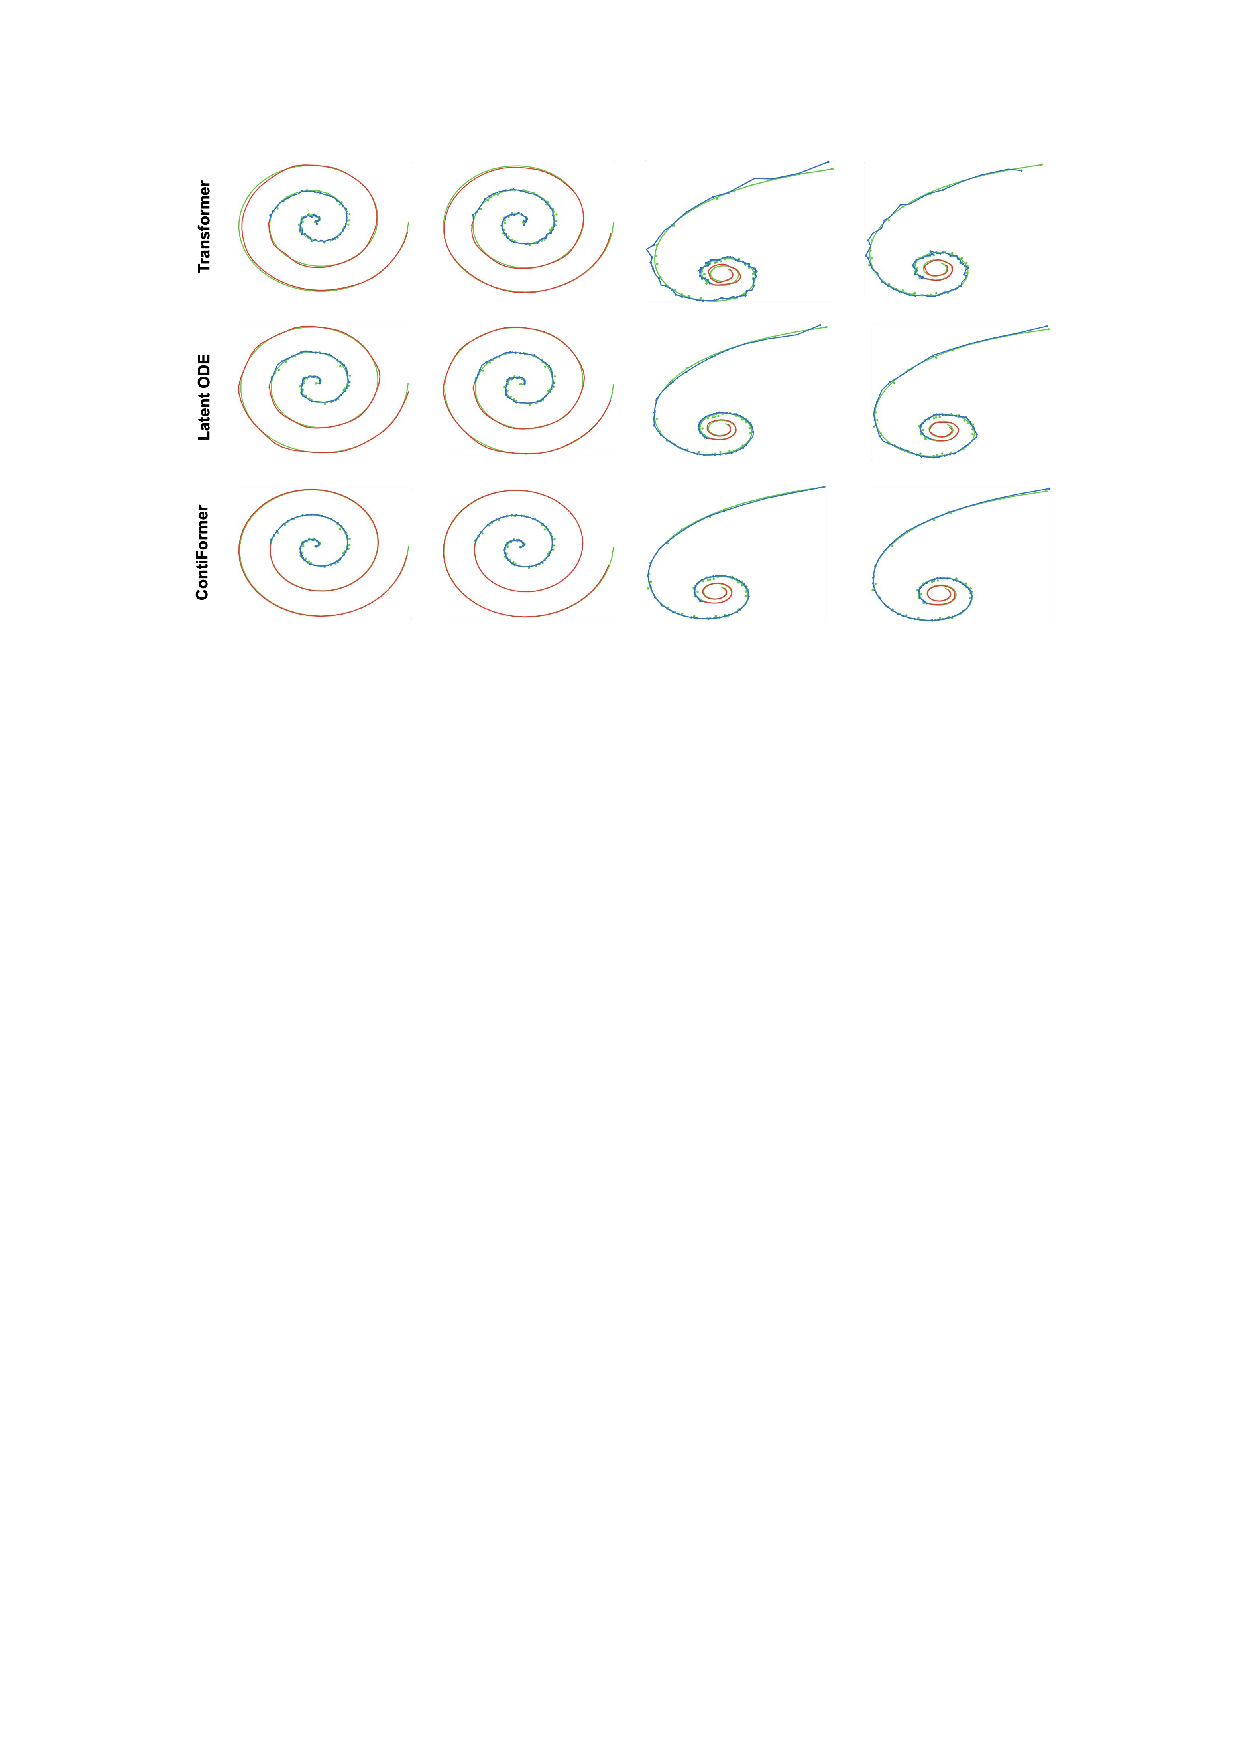
\includegraphics[width=\textwidth]{fig/interpolation_full.pdf}
    \caption{More visualization results with $\alpha=0.02$. Here, Latent ODE refers to Latent ODE w/ RNN Encoder~\cite{chen2018neural}.}
    \label{fig:int2}
\end{figure}

\subsection{Irregular Time Series Classification} \label{sec:classify}

\subsubsection{Training Details}

For both our model and the baseline models, we adopted a fixed learning rate of $10^{-2}$ and a batch size of $64$. To ensure the reliability of our results, all experiments were conducted three times, and the reported values represent the mean. The training process for all models lasted for 1000 epochs. However, if the training accuracy failed to show any improvement for 100 consecutive epochs, the training was stopped to avoid unnecessary computation. 

\subsubsection{Dataset Information}

We select 20 datasets from UEA Time Series Classification Archieve with diverse characteristics in terms of the number, dimensionality and length of time series samples, as well as the number of classes. Detailed information is listed in Table \ref{tab:ueadata}.

\begin{table*}[htbp]
    \centering
    \caption{Dataset Information of UEA.}
    \resizebox{\textwidth}{!}{%
    \begin{tabular}{ccccccc}
    \toprule
         Dataset & Ablation & \# Train & \# Test & Length & \# Classes & \# Variates    \\
    \midrule
ArticularyWordRecognition & AWR &  275 &	300 &	144 &	25 &	9  \\
BasicMotions & BM & 40 & 	40 &	100 &	4 &	6 \\
CharacterTrajectories & CT & 1422 &	1436 &	182 &	20 &	3 \\
DuckDuckGeese & DDG & 60 &	40 &	270 &	5 &	1345 \\
Epilepsy & EP & 137 &	138 &	207 &	4 &	3 \\
ERing & ER & 30 &	270 &	65 &	6 &	4 \\
FingerMovements & FM & 316 &	100 &	50 &	2 &	28\\
HandMovementDirection & HMD & 160 &	74 &	400 &	4 &	10 \\
Handwriting & HW & 150 & 	850 & 	152 & 	26 &	3 \\
Heartbeat & HB & 204 &	205 &	405 &	2 &	61 \\
JapaneseVowels & JV & 270 &	370 &	29 &	9 &	12 \\
Libras & LB & 180 &	180 &	45 &	15 &	2 \\
LSST & LSST & 2459 &	2466 &	36 &	14 &	6\\
NATOPS & NATOPS & 180 &	180 &	51 &	6 & 	24 \\
PEMS-SF & PEMS & 267 &	173 &	144 &	7 &	963 \\
PenDigits & PD & 7494 &	3498 &	8 &	10 &	2 \\
RacketSports & RS & 151 &	152 &	30 &	4 &	6 \\
SelfRegulationSCP1 & SR & 268 &	293 &	896 &	2 &	6 \\
SpokenArabicDigits & SA & 6599 &	2199 &	93 &	10 &	13 \\
UWaveGestureLibrary & UGL & 2238 &	2241 &	315 &	8 &	3 \\
\bottomrule
    \end{tabular}}
    \label{tab:ueadata}
\end{table*}

\subsubsection{Full Experimental Results} \label{sec:full}

We follow the setting of \cite{kidger2020neural} to randomly drop either 30\%, 50\% or 70\% observations. Experimental results are shown in Table \ref{tab:uea30}, Table \ref{tab:uea50} and Table \ref{tab:uea70}. We can find that ContiFormer outperforms RNN-based methods, ODE-based methods and Transformer-based methods. Also, we observe that ContiFormer outperforms all the baselines by a large margin when 70\% observations are dropped, which confirms that ContiFormer is more suitable for irregular time series modeling.

\begin{table*}[htbp]
\centering
\caption{Experimental result on UEA when 30\% observations are dropped. (ODE. stands for ODE-RNN, N. CDE stands for Neural CDE, ACC. stands for Accuracy.)}
\resizebox{\textwidth}{!}{%
\begin{tabular}{cccccccccc}
\toprule
Dataset & GRU-D & GRU-$\Delta$t      & ODE. & CADN    & N. CDE &  S5  & mTAN & TST        & \textbf{ContiFormer} \\
\midrule
        AWR & 0.8533  & 0.8956  & 0.8789  & 0.8056  & 0.9089  & 0.9011  & 0.8067  & \textbf{0.9722}  & 0.9633  \\ 
        BM & 0.9333  & 0.9417  & 0.8250  & 0.9583  & \textbf{0.9917}  & 0.9833  & \textbf{0.9917}  & 0.9667  & 0.9750  \\ 
        CT & 0.9325  & 0.8558  & 0.9415  & 0.9575  & 0.9276  & 0.9610  & 0.9529  & 0.9742  & \textbf{0.9833}  \\ 
        DDG & 0.5867  & 0.5933  & 0.5067  & 0.4600  & 0.3400  & 0.5667  & 0.6000  & 0.6533  & \textbf{0.7267}  \\ 
        EP & 0.7995  & 0.8043  & 0.8454  & 0.8123  & 0.7657  & 0.9074  & 0.9203  & \textbf{0.9589}  & 0.9324  \\ 
        ER & 0.7062  & 0.7148  & 0.6296  & 0.8623  & 0.7543  & 0.8346  & 0.7123  & 0.9160  & \textbf{0.9210}  \\
        FM & 0.6167  & 0.6167  & 0.5667  & \textbf{0.6233}  & 0.5867  & 0.6033  & 0.5433  & 0.6133  & 0.6000  \\ 
        HMD & 0.3559  & 0.4099  & 0.5450  & 0.4505  & 0.3333  & \textbf{0.6171}  & 0.4414  & 0.5946  & 0.4550  \\ 
        HW & 0.0722  & 0.1251  & 0.0675  & 0.0925  & 0.1831  & 0.1302  & 0.0937  & \textbf{0.2196}  & 0.2000  \\ 
        HB & 0.7577  & 0.7593  & 0.7805  & 0.7431  & 0.7333  & 0.7431  & \textbf{0.7789}  & 0.7398  & 0.7561  \\ 
        JV & 0.9703  & 0.9550  & 0.9432  & 0.9703  & 0.9225  & 0.9676  & 0.9595  & 0.9865  & \textbf{0.9919}  \\ 
        LB & 0.5037  & 0.4741  & 0.5222  & 0.5938  & 0.7481  & \textbf{0.9216}  & 0.5426  & 0.7519  & 0.8778  \\
        LSST & 0.5589  & 0.5615  & 0.5715  & 0.5574  & 0.3940  & \textbf{0.6389}  & 0.5307  & 0.5520  & 0.6004  \\ 
        NATOPS & 0.9204  & 0.9315  & 0.8704  & 0.8944  & 0.8148  & 0.8500  & 0.9019  & \textbf{0.9352}  & 0.9222  \\ 
        PEMS & 0.7938  & 0.7669  & 0.8208  & 0.7958  & 0.7572  & 0.9133  & 0.8189  & \textbf{0.8420}  & 0.8401  \\ 
        PD & 0.9309  & 0.9222  & 0.9433  & 0.9402  & 0.8422  & 0.8110  & 0.9029  & \textbf{0.9520}  & 0.9517  \\ 
        RS & 0.7434  & 0.7281  & 0.7654  & 0.7325  & 0.6798  & 0.7500  & 0.7325  & 0.8158  & \textbf{0.8487}  \\ 
        SR & 0.8942  & \textbf{0.9124}  & 0.9101  & 0.8259  & 0.8783  & 0.8737  & 0.8646  & 0.9044  & 0.9101  \\ 
        SA & 0.9663  & 0.9660  & 0.9830  & 0.9809  & 0.8998  & 0.9291  & 0.9321  & 0.9744  & \textbf{0.9836}  \\ 
        UGL & 0.6729  & 0.6625  & 0.6917  & 0.7479  & 0.8219  & 0.8042  & 0.7344  & \textbf{0.8552}  & 0.8135  \\ 
    \midrule
        \textbf{Acc.} ($\uparrow$) & 0.7284  & 0.7298  & 0.7304  & 0.7402  & 0.7142  & 0.7854  & 0.7381  & 0.8089  & \textbf{0.8126}  \\
        \textbf{Rank}  ($\downarrow$) & 6 & 5.75 & 5.45 & 5.4 & 6.85 & 4.4 & 5.7 & 2.75 & \textbf{2.4} \\ 
\midrule
\bottomrule
\end{tabular}}
\label{tab:uea30}
\end{table*}

\begin{table*}[htbp]
\centering
\caption{Experimental result on UEA when 50\% observations are dropped. (ODE. stands for ODE-RNN, N. CDE stands for Neural CDE, ACC. stands for Accuracy.)}
\resizebox{\textwidth}{!}{%
\begin{tabular}{cccccccccc}
\toprule
Dataset & GRU-D & GRU-$\Delta$t      & ODE.  & CADN   & N. CDE & S5  & mTAN & TST        & \textbf{ContiFormer} \\
\midrule
AWR & 0.8811  & 0.8978  & 0.8989  & 0.8067  & 0.9133  & 0.9078  & 0.8067  & \textbf{0.9633}  & \textbf{0.9633}  \\ 
BM & 0.9417  & 0.8500  & 0.7667  & 0.9417  & 0.9583  & \textbf{0.9917}  & 0.9583  & 0.9500  & 0.9583  \\ 
CT & 0.8872  & 0.9088  & 0.9506  & \textbf{0.9798}  & 0.9285  & 0.9638  & 0.9431  & 0.9601  & \textbf{0.9798}  \\ 
DDG & 0.5467  & 0.6000  & 0.4933  & 0.5467  & 0.3467  & 0.5667  & 0.6067  & 0.6533  & \textbf{0.6867}  \\
EP & 0.7295  & 0.7899  & 0.7512  & 0.6728  & 0.7101  & 0.9012  & 0.9106  & \textbf{0.9589}  & 0.9469  \\ 
ER & 0.7358  & 0.7432  & 0.5704  & 0.8527  & 0.7691  & 0.8284  & 0.6432  & \textbf{0.9012}  & 0.8901  \\ 
FM & 0.5800  & 0.5967  & 0.5933  & 0.5933  & 0.6000  & 0.6033  & 0.5700  & \textbf{0.6067}  & \textbf{0.6067}  \\
HMD & 0.4099  & 0.4054  & 0.4685  & 0.4550  & 0.3243  & \textbf{0.5811}  & 0.4099  & 0.5270  & 0.4595  \\ 
HW & 0.0769  & 0.0945  & 0.0588  & 0.1004  & 0.1855  & 0.1357  & 0.0737  & 0.1600  & \textbf{0.1757}  \\ 
HB & 0.7642  & 0.7593  & \textbf{0.7707}  & 0.7512  & 0.7333  & 0.7463  & 0.7789  & 0.7350  & 0.7610  \\ 
JV & 0.9604  & 0.9532  & 0.9126  & 0.9649  & 0.9180  & 0.9631  & 0.9595  & 0.9775  & \textbf{0.9856}  \\ 
LB & 0.3796  & 0.4352  & 0.4537  & 0.5680  & 0.7315  & 0.6352  & 0.5259  & 0.6556  & \textbf{0.8537}  \\ 
LSST & 0.5203  & 0.5292  & 0.5223  & 0.5222  & 0.3969  & \textbf{0.7204}  & 0.5126  & 0.5151  & 0.5661  \\ 
NATOPS & 0.9185  & 0.9167  & 0.8444  & 0.8741  & 0.8019  & 0.8315  & 0.8778  & 0.8778  & \textbf{0.9222}  \\ 
PEMS & 0.7823  & 0.7861  & 0.8170  & 0.7611  & 0.7534  & \textbf{0.9114 } & 0.8015  & 0.7669  & 0.8401  \\
PD & 0.8245  & 0.7804  & 0.8563  & 0.8369  & 0.6389  & 0.6544  & 0.6898  & \textbf{0.8827}  & 0.8799  \\ 
RS & 0.7412  & 0.7368  & 0.7127  & 0.7632  & 0.5526  & 0.7193  & 0.6601  & 0.7807  & \textbf{0.8355}  \\ 
SR & 0.9135  & \textbf{0.9170}  & 0.9044  & 0.8123  & 0.8760  & 0.8885  & 0.8658  & 0.8987  & 0.9067  \\ 
SA & 0.9583  & 0.9556  & 0.9759  & 0.9663  & 0.8907  & 0.9218  & 0.9254  & 0.9667  & \textbf{0.9767}  \\ 
UGL & 0.6833  & 0.6583  & 0.6781  & 0.6531  & 0.8281  & 0.8042  & 0.7167  & \textbf{0.8490}  & 0.8000  \\ 
\midrule
\textbf{ACC.} ($\uparrow$) & 0.7117  & 0.7157  & 0.7000  & 0.7211  & 0.6929  & 0.7638  & 0.7118  & 0.7793  & \textbf{0.7997} \\ 
\textbf{Rank}  ($\downarrow$) & 5.8 & 5.65 & 5.75 & 5.55 & 6.5 & 4.25 & 5.85 & 3.15 & \textbf{1.9} \\ 
\bottomrule
\end{tabular}}
\label{tab:uea50}
\end{table*}

\begin{table*}[t]
\centering
\caption{Experimental result on UEA when 70\% observations are dropped. (ODE. stands for ODE-RNN, N. CDE stands for Neural CDE, ACC. stands for Accuracy)}
\resizebox{\textwidth}{!}{%
\begin{tabular}{cccccccccc}
\toprule
Dataset & GRU-D & GRU-$\Delta$t      & ODE.  & CADN   & N. CDE  & S5 & mTAN & TST  & \textbf{ContiFormer} \\
\midrule
AWR & 0.8689  & 0.8822  & 0.8433  & 0.7911  & 0.9178  & 0.8956  & 0.7956  & 0.9089  & \textbf{0.9511}  \\ 
        BM & 0.7583  & 0.7917  & 0.7167  & \textbf{0.9750}  & 0.9000  & 0.9167  & 0.9417  & 0.9167  & 0.9167  \\ 
        CT & 0.8433  & 0.8496  & 0.9471  & 0.9582  & 0.9241  & 0.9547  & 0.9009  & 0.9313  & \textbf{0.9675}  \\ 
        DDG & 0.5200  & 0.6000  & 0.4800  & 0.5667  & 0.3533  & 0.5667  & 0.6067  & 0.5867  & \textbf{0.7267}  \\ 
        EP & 0.7464  & 0.7222  & 0.6643  & 0.6667  & 0.6667  & 0.8802  & 0.9058  & \textbf{0.9420}  & 0.9275  \\ 
        ER & 0.6741  & 0.6617  & 0.5383  & \textbf{0.8647}  & 0.7630  & 0.8025  & 0.7407  & 0.8198  & 0.8580  \\ 
        FM & 0.5467  & 0.5933  & 0.5733  & 0.6000  & 0.5767  & 0.6133  & 0.5700  & 0.5300  & \textbf{0.6233}  \\
        HMD & 0.3829  & 0.3784  & 0.4459  & 0.4324  & 0.3378  & \textbf{0.5991}  & 0.3694  & 0.4324  & 0.4144  \\
        HW & 0.0784  & 0.0831  & 0.0541  & 0.0957  & \textbf{0.1533}  & 0.1078  & 0.0604  & 0.1255  & 0.1247  \\
        HB & 0.7610  & 0.7528  & 0.7593  & 0.7610  & 0.7561  & 0.7512  & \textbf{0.7691}  & 0.7593  & 0.7593  \\ 
        JV & 0.9514  & 0.9414  & 0.9261  & 0.9685  & 0.8964  & 0.9559  & 0.9613  & 0.9595  & \textbf{0.9766}  \\ 
        LB & 0.3648  & 0.3722  & 0.3463  & 0.5412  & 0.6796  & 0.6278  & 0.4926  & 0.5500  & \textbf{0.7648}  \\ 
        LSST & 0.4803  & 0.4895  & 0.4505  & \textbf{0.5278}  & 0.4093  & 0.6778  & 0.4992  & 0.4874  & 0.5149  \\ 
        NATOPS & 0.8722  & 0.8981  & 0.7889  & 0.9074  & 0.7944  & 0.8259  & 0.8463  & 0.8315  & \textbf{0.9204}  \\ 
        PEMS & 0.7418  & 0.7611  & 0.7842  & 0.7726  & 0.7303  & \textbf{0.8902}  & 0.7861  & 0.6840  & 0.8227  \\ 
        PD & 0.7451  & 0.6670  & 0.7802  & 0.7596  & 0.5201  & 0.5197  & 0.6063  & \textbf{0.8078}  & 0.8069  \\ 
        RS & 0.6711  & 0.6776  & 0.6316  & 0.7018  & 0.5570  & 0.6382  & 0.6228  & 0.6930  & \textbf{0.7697}  \\ 
        SR & 0.9090  & \textbf{0.9170}  & 0.9158  & 0.8515  & 0.8726  & 0.8874  & 0.8635  & 0.8612  & 0.8953  \\ 
        SA & 0.9304  & 0.9295  & 0.9523  & 0.9513  & 0.8622  & 0.9024  & 0.8925  & 0.9447  & \textbf{0.9600}  \\
        UGL & 0.6031  & 0.6219  & 0.5896  & 0.6729  & \textbf{0.8344}  & 0.7896  & 0.6792  & 0.8219  & 0.7969  \\
    \midrule
        \textbf{ACC.} ($\uparrow$) & 0.6725  & 0.6795  & 0.6594  & 0.7183  & 0.6753  & 0.7401  & 0.6955  & 0.7297  & \textbf{0.7749}  \\ 
        \textbf{Rank}  ($\downarrow$) & 6.15 & 5.7 & 6.4 & 3.9 & 6.3 & 4.45 & 5.4 & 4.2 & \textbf{2.1} \\
\bottomrule
\end{tabular}}
\label{tab:uea70}
\end{table*}

\subsection{Predicting Irregular-Sampled Sequences} \label{sec:mtpp}

\subsubsection{Background: Marked Temporal Point Process (MTPP)}

The marked Temporal Point Process (MTPP) has been widely studied in recent years. We define a sequence of events and types as $\Gamma=[(t_1, k_1), (t_2, k_2), \ldots, (t_N, k_N)]$, where $t_i$ is the time point when the $i$-th event occurs, with $t_1 < t_2 < \ldots < t_N$, $k_i \in \{ 1, 2, \ldots, \mathcal{K} \}$ is the type of the $i$-th event and $\mathcal{K}$ is the total number of event types. A history event is the event sequence up to but not including time $t$, denoted by $\mathcal{H}_t={(t_j, k_j): t_j<t}$. The goal of the temporal point process is to model the conditional intensity function (CIF), denoted by $\lambda_{k}^{*}(t)$, which represents the likelihood of an event occurring at time $t$, given the historical events. Models are trained so that the log probability of an event sequence, i.e., 

\begin{equation}
    \log p(\Gamma)=\sum_{j=1}^N \log \lambda_{k_j}^*\left(t_j\right)-\int_{t_1}^{t_N} \lambda^*(\tau) d \tau ~.
\end{equation}

\subsubsection{Dataset Description} 

We use one synthetic dataset and five real-world datasets, namely Synthetic, Neonate~\cite{stevenson2019dataset}, Traffic~\cite{lai2018modeling},
MIMIC~\cite{du2016recurrent}, BookOrder~\cite{du2016recurrent} and StackOverflow~\cite{leskovec2014snap} to evaluate our model. 

\paragraph{Synthetic}

To evaluate the effectiveness of the proposed method, we create a synthetic dataset. Specifically, we consider $10$ types of event where each type of event contain three properties, i.e., $(X_i, V_i, D_i)$. Hence, given an event $\textbf{e}$ with type $j$ is represented as $\textbf{e} = (e.x, e.v, e.d, e.k)$, where $e.x \sim \mathcal{N}(X_j, \mu_1)$, $e.v \sim \mathcal{N}(V_j, \mu_2)$, $e.d=D_j > 0 $ and $e.k$ is the type of the event. We set $\mu_1=\mu_2=0.01$ and $X, V, D \in \mathbb{R}^{10}$ is randomly generated and pre-defined.

To model both the correlation between events and the dynamic changes of events within the system. We first define the dynamic attention (weight) for each event, which is composed of inter-event dependency modeling and intra-event dynamic modeling. For inter-event dependency, it aims to calculate time-aware attention (weight) between each pair of events. Specifically, we use the following equation to define the weight between event $\textbf{e}$ and $\hat{\textbf{e}}$,
\begin{equation}
    \omega(\textbf{e}, \hat{\textbf{e}}) = (e.t - \hat{e}.t) \cdot (e.x * \hat{e}.v - \hat{e}.x * e.v) ~.
\end{equation}
Next, the define $\lambda_{k}^{*}(t)$ and $\lambda^{*}(t)$ in which we assume that only the last event attributes to the decision of the next event, following Markov decision process (MDP), i.e.

\begin{equation}
\begin{aligned}
\lambda_{k}^{*}(t) & = P(k | \hat{e}.k) \cdot \text{Softplus} \left(\sum_{\textbf{e} \in \mathcal{H}_t} \omega(\textbf{e}, \hat{\textbf{e}}) \cdot \text{exp} \left( \frac{- (t - e.t)}{e.d} \right) \right) ~,\\
\lambda^{*}(t) & = \text{Softplus} \left(\sum_{\textbf{e} \in \mathcal{H}_t} \omega(\textbf{e}, \hat{\textbf{e}}) \cdot \text{exp} \left( \frac{- (t - e.t)}{e.d} \right) \right) ~.\\
\end{aligned}
\label{eq:lam}
\end{equation}
where $\text{exp} \left( - (t - e.t) / e.d \right)$ is the exponential decay effect for each event, $\hat{\textbf{e}}$ is the last event as of time $t$. The existence of the exponential decay function ensures that all the events will eventually disappear in the system as time goes to infinity so as to stabilize the conditional intensify function. $P(k | \hat{k})$ is a pre-defined matrix that means the probability of the next event to with type $k$ given that the type of the previous event is $\hat{\textbf{e}}$.

Next, we predict the occurrence time of the next event with
\begin{equation}
    \begin{aligned}
        \widehat{t}_{j+1} & =\int_{t_j}^{\infty} t \cdot p\left(t \mid \mathcal{H}_t\right) d t ~,\\
        \text{ where \quad} p\left(t \mid \mathcal{H}_t\right) & =\lambda^{*}(t) \exp \left(-\int_{t_j}^t \lambda^{*}(t) d t\right) ~.\\
    \end{aligned}
    \label{eq:pre}
\end{equation}
To predict the type of the next event, we sample the type of the next event from $P(\cdot | \hat{e}.k)$, where $\hat{e}.k$ is the type of the previous event.

Finally, we use 500 different random seeds to generate a total of 500 event sequences. Also, we use 4-fold cross-validation for evaluation. The generation process is shown in Algorithm \ref{algo:gen}.

\begin{algorithm}
\caption{Generate Synthetic Dataset with Time-Aware Dynamic Kernel}
\label{algo:gen}
\begin{algorithmic} 
\STATE \textbf{Input} $\textit{seed} \in [0, 500)$, $\textit{tmax}=20$, $X = [0.78, 0.11, -1.0, -0.56, -0.78, 1.0, 0.56, -0.33, 0.3, $ $-0.11]$, $V=[-0.17, 0.5, -0.28, 0.28, 0.17, 0.39, -0.05, 0.05, -0.39, -0.5]$, $D=[0.5, 0., 0.28, $ $ 0.17, 0.22, 0.44, 0.33, 0.11, 0.05, 0.39]$ 

\STATE \textbf{Output} A generated event sequence $E$. 

\STATE Initialize the random state of Numpy using $\textit{seed}$ and defined the probabilistic matrix $P$.  
\STATE Initialize the event sequence $E$ to be an empty array, and set current time $T=0$.
\STATE Random generate the type of the first event $e.k$ and sample $e.x, e.v$ and $e.d$.
\STATE Add the event to the event sequence.
\WHILE {$ t \leq \textit{tmax}$}
    \STATE Calculate the conditional intensity function using Eq. (\ref{eq:lam}).
    \STATE Predict the time of the next event $e.t$ using Eq. (\ref{eq:pre}).
    \STATE Assume the type of previous event is $\hat{k}$, sample the type of the next event $e.k$ from $P(\cdot | \hat{k})$.
    \STATE Sample sample $e.x, e.v$ and $e.d$ given $e.k$.
    \STATE Add the generated event to the event sequence $E$.
    \STATE Update $T=e.t$.
\ENDWHILE
\RETURN $E$
\end{algorithmic}
\end{algorithm}

\paragraph{Neonate.} Neonate dataset is a clinical dataset from 79 patients, among which 48 patients have incurred at least two seizures during the observation. The dataset contains only one type of event, i.e., the start point of a seizure (in minutes). The task is to predict when the next seizure will happen. Note that we only clear the start point of the seizure. Thus, we only have one type of event.

\paragraph{Traffic.} Traffic dataset is a benchmark dataset for time-series forecasting collected by the Caltrans Performance Measurement System (PeMS). This dataset contains the traffic state monitoring of 861 sensors in a two-year period. The data is collected every 1 hour. We extract time points with fluctuations higher than 50\% as events, whose types are up and down according to the direction. We consider two events that are within 6 hours as duplicated events and remove the latter one from the dataset. Besides, for each sensor, it contains a long sequence, we partition these event sequences by month, i.e., for each event sequence, it contains the event of a sensor in one month.

\paragraph{MIMIC.} MIMIC dataset is a clinical dataset that collects patients' visits to a hospital's ICU in a seven-year period. We treat the visits of each patient as a separate sequence.

\paragraph{BookOrder.} BookOrder dataset is a financial dataset that contains transaction records of stock in one day. We record the time (in milliseconds) and the action that was taken in each transaction. The dataset is a single long sequence with only two types of events: “buy” and “sell”. We clip the event sequences so that the maximum length is 500 in both the train and test sets. Furthermore, the mean $\mu$ and standard derivative $\sigma$ of the time difference between two events in the dataset is 1.32 and 20.24 respectively. Therefore, we clip the maximum time difference to 70.

\paragraph{StackOverflow.} StackOverflow dataset is a question-answering website. The website rewards users with badges to promote engagement in the community, and the same badge can be rewarded multiple times to the same user. We collect data in a two-year period, and we treat each user’s reward history as a sequence.

For MIMIC, Bookorder, and StackOverflow datasets, we use the dataset from the Google Drive\footnote{\url{https://drive.google.com/drive/folders/0BwqmV0EcoUc8UklIR1BKV25YR1U?resourcekey=0-OrlU87jyc1m-dVMmY5aC4w}}. Statistic information can be found in Table ~\ref{tab:data}. We use the 4-fold cross-validation scheme for Synthetic, Neonate, and Traffic datasets following~\cite{fang2023learning}, and the 5-fold cross-validation scheme for the other three datasets following~\cite{mei2017neural, zuo2020transformer}.


\begin{table*}[htbp]
    \centering
    \caption{Dataset statistics: name of the dataset, number of event types, number of events in the dataset, average length per sequence, and number of sequences in training/test sets.}
    \begin{tabular}{c|c|c|c|c|c}
    \toprule
         Dataset & K & \# Events & Avg. Length & \# Train Seqs & \# Test Seqs  \\
    \midrule
         Synthetic & 10 & 8, 618 & 17 & 375 & 125\\
         Neonate & 1 & 534 & 11 & 38 & 10 \\
         Traffic & 2 & 154, 747 & 60 & 1, 938 & 647 \\
         MIMIC & 75 & 2, 419 & 4 & 527 & 65 \\
         BookOrder & 2 & 414, 800 & 2, 074 & 90 & 100 \\
         StackOverflow & 22 & 480, 413 & 72 & 4, 777 & 1, 326 \\
    \bottomrule
    \end{tabular}
    \label{tab:data}
\end{table*}

\subsubsection{Implementation Details} 

\paragraph{Input Embedding}

Given the history event $\mathcal{H}_t=\left\{\left(t_j, k_j\right): t_j<t\right\}$ with a total of $\mathcal{K}$ events, the input of Transformer-based model and RNN-based model is obtained through event embedding and temporal encoding, i.e., for the $i$-th event $x_i = \text{emb}(k) + \text{enc}(t)$, where $\text{emb}(k)$ is the $k$-th column of the embedding table $\mathcal{E} \in \mathbb{R}^{\mathcal{K} \times d}$ and temporal encoding is defined by a combination of sine and cosine function~\cite{zuo2020transformer}.

\paragraph{Conditional Intensity Function}

Given the output from the model, i.e. $\mathbf{h}\left(t_1\right), \mathbf{h}\left(t_2\right),  .., \mathbf{h}\left(t_N\right)$. The dynamics of the temporal point process are described by a continuous conditional intensity function. To reduce the memory cost and accelerate the training process. Instead of using the continuous-time output from ContiFormer, we only use ContiFormer to generate a hidden representation for discrete time points, i.e., $t_1, t_2, ..., t_j, ..., t_N$. Following ~\cite{zuo2020transformer}, the conditional intensity function is defined by
\begin{equation}
\lambda\left(t \mid \mathcal{H}_t\right)=\sum_{k=1}^K \lambda_k\left(t \mid \mathcal{H}_t\right) ~,
\end{equation}
where each of the type-specific conditional intensity function is defined by
\begin{equation}
\lambda_k\left(t \mid \mathcal{H}_t\right)=f_k\left(\alpha_k \frac{t-t_j}{t_j}+\mathbf{w}_k^{\top} \mathbf{h}\left(t_j\right)+b_k\right) ~,
\end{equation}
where on interval $t \in [t_j, t_{j+1})$ and $f_k(x)=\beta_k \log \left(1+\exp \left(x / \beta_k\right)\right)$ is the softplus function with parameter $\beta_k$. The use of such a closed-form intensity function allows for $O(1)$ interpolation.

\paragraph{Training Loss} \label{sec:loss}

We train our model and all the baseline models by jointing maximizing the log-likelihood of the sequence and minimizing the prediction losses.

Specifically, for a sequence $\mathcal{S}$ over an interval $[t_i, t_N]$, given the conditional intensity function $\lambda\left(t \mid \mathcal{H}_t\right)$, the log-likelihood is given by
\begin{equation}
\ell_{LL}(\mathcal{S})=\underbrace{\sum_{j=1}^N \log \lambda\left(t_j \mid \mathcal{H}_j\right)}_{\text {event log-likelihood }}-\underbrace{\int_{t_1}^{t_N} \lambda\left(t \mid \mathcal{H}_t\right) d t}_{\text {non-event log-likelihood }} .
\end{equation}
One challenge to compute the log-likelihood is to solve the integral, i.e., $\Lambda=\int_{t_1}^{t_N} \lambda\left(t \mid \mathcal{H}_t\right) d t$. Since \textit{softplus} function has no closed-form computation, we apply the Monte Carlo integration method, i.e.,
\begin{equation}
\widehat{\Lambda}_{\mathrm{MC}}=\sum_{j=2}^P\left(t_j-t_{j-1}\right)\left(\frac{1}{P} \sum_{i=1}^P \lambda\left(u_i\right)\right) ~,
\end{equation}
where $u_i \sim \operatorname{Unif}(t_{j-1}, t_j)$ for $i \in [1, ..., P]$ is sampled from a uniform distribution over an interval $[t_{j-1}, t_j]$.

Besides the log-likelihood loss, we also use the cross-entropy loss and regression loss for predicting the type and time of the next events.

Specifically, given the conditional intensity function, the next time stamp prediction is given by
\begin{equation}
\begin{aligned}
& p\left(t \mid \mathcal{H}_t\right)=\lambda\left(t \mid \mathcal{H}_t\right) \exp \left(-\int_{t_j}^t \lambda\left(\tau \mid \mathcal{H}_\tau\right) d \tau\right) ~, \\
& \widehat{t}_{j+1}=\int_{t_j}^{\infty} t \cdot p\left(t \mid \mathcal{H}_t\right) d t ~. \\
\end{aligned}
\end{equation}
Thus, the regression loss and the cross-entropy loss are given by
\begin{equation}
\ell_{reg}(\mathcal{S}) = \sum_{i=2}^{N} (\widehat{t}_{i} - t_i)^2 ~, 
\ell_{pred}(\mathcal{S}) = \sum_{i=2}^{N} -\log \left( \frac{\lambda_{k_i}\left(\widehat{t}_{i}\right)}{\lambda\left(\widehat{t}_{i} \right)} \right) ~.
\end{equation}
Overall, the modeling is trained in a multi-task manner, i.e., 
\begin{equation}
    \ell(\mathcal{S}) = \ell_{LL} + \alpha_1 \ell_{reg}(\mathcal{S}) + \alpha_2 \ell_{pred}(\mathcal{S}) ~,
\end{equation}
where $\alpha_1$ and $\alpha_2$ are the pre-defined weight. By default, we set $\alpha_1=0.01$ and $\alpha_2=1$.

\subsubsection{Significance test on Synthetic and BookOrder datasets}

To demonstrate the statistical superiority of ContiFormer, we conducted a t-test on Synthetic and BookOrder datasets using 10 random seeds. The t-test results are listed in Table \ref{tab:ttest}.

\begin{table}[htbp]
    \centering
    \caption{Significance test on Synthetic and BookOrder dataset with 10 repeats. The P-value represents the significant value between the ContiFormer and the baseline model. Bolder values represent P-value $< 10^{-6}$ in significance test.}
    \resizebox{\textwidth}{!}{%
    \begin{tabular}{ccccccccccccc}
    \toprule
        Dataset & \multicolumn{6}{c}{Synthetic} & \multicolumn{6}{c}{BookOrder} \\
        \cmidrule(lr){2-7}
        \cmidrule(lr){8-13}
        Metric & \multicolumn{2}{c}{LL ($\uparrow$)} & \multicolumn{2}{c}{Accuracy ($\uparrow$)} & \multicolumn{2}{c}{RMSE ($\downarrow$)} & \multicolumn{2}{c}{LL ($\uparrow$)} & \multicolumn{2}{c}{Accuracy ($\uparrow$)} & \multicolumn{2}{c}{RMSE ($\downarrow$)} \\ 
        \cmidrule(lr){2-3}
        \cmidrule(lr){4-5}
        \cmidrule(lr){6-7}
        \cmidrule(lr){8-9}
        \cmidrule(lr){10-11}
        \cmidrule(lr){12-13}
        Statistic & Mean & P-value & Mean & P-value & Mean & P-value & Mean & P-value & Mean & P-value & Mean & P-value \\ 
    \midrule
        GRU-dt & -0.8611 & 5.38E-08 & 0.8420 & 0.003 & 0.2556 & 3.49E-09 & -1.0137 & 1.07E-31 & 0.6274 & 3.11E-08 & 3.6680 & 1.32E-05 \\ 
        NSTKA & -1.0088 & 1.27E-21 & 0.8419 & 0.0003 & 0.3863 & 1.74E-12 & -1.0916 & 2.95E-27 & 0.6223 & 5.48E-15 & 3.7175 & 1.88E-08 \\ 
        ODE-RNN & -0.8432 & 2.39E-11 & 0.8420 & 0.098 & 0.2401 & 3.77E-08 & -0.9458 & 1.44E-26 & 0.6278 & 1.17E-07 & 3.5898 & 1.94E-03 \\ 
        RMTPP & -1.0132 & 3.57E-19 & 0.8420 & 0.0143 & 0.3711 & 6.70E-18 & -0.9551 & 9.70E-26 & 0.6245 & 1.45E-13 & 3.6475 & 9.76E-04 \\ 
        SAHP & -0.6247 & 2.21E-05 & 0.8420 & 0.1778 & 0.5218 & 2.37E-10 & -0.3053 & 1.83E-07 & 0.6227 & 1.45E-13 & 3.6810 & 9.55E-07 \\ 
        THP & -0.6035 & 6.28E-06 & 0.8420 & 0.1354 & 0.2100 & 4.85E-06 & -1.0788 & 1.55E-17 & 0.6251 & 1.96E-06 & 3.6907 & 8.02E-07 \\
    \midrule
        ContiFormer & \textbf{-0.5445} & N/A & 0.8421 & N/A & \textbf{0.1943} & N/A & \textbf{-0.2745} & N/A & \textbf{0.6295} & N/A & 3.6171 & N/A \\
    \bottomrule
    \end{tabular}}
    \label{tab:ttest}
\end{table}

\subsection{Regular Time Series Forecasting} \label{sec:regular}

Time series forecasting has garnered considerable attention in recent years, as evidenced by various studies~\cite{wu2021autoformer, zhou2021informer, li2023towards}. In this study, we assess ContiFormer against several models tailored for regular time series forecasting. 

\paragraph{Datasets}

We evaluate ContiFormer on five experimental datasets. i) ETT dataset \cite{zhou2021informer} contains the data collected from electricity transformers, including load and oil temperature that are recorded every 15 minutes between July 2016 and July 2018. Here, we use ETTm2 and ETTh2 datasets. ii) Exchange dataset \cite{wu2021autoformer} records the daily exchange rates of eight different countries ranging from 1990 to 2016. iii) Weather dataset is recorded every 10 minutes for 2020 whole year, which contains 21 meteorological indicators, such as air temperature, humidity, etc. v) ILI dataset includes the weekly recorded influenza-like illness (ILI) patients data from Centers for
Disease Control and Prevention of the United States between 2002 and 2021. 

\paragraph{Baselines}

We compare ContiFormer with several transformer-based models for regular time series forecasting under the multivariate setting. These transformer-based models includes: FEDformer\cite{zhou2022fedformer}, Autoformer\cite{wu2021autoformer}, Informer\cite{zhou2021informer} and Reformer\cite{kitaev2020reformer}. Also, we chose one recent state-of-the-art model. i.e. TimesNet\cite{wu2022timesnet} for comparison.

\paragraph{Results of Time Series Forecasting}

The experimental results are depicted in Table~\ref{tab:regular}. ContiFormer achieves the best performance on ILI dataset. Specifically, it gives \textbf{10\%} MSE reduction (2.874 $\rightarrow$ 2.632). Also, ContiFormer outperforms Autoformer and FEDformer on Exchange, ETTm2, and Weather datasets. Therefore, it demonstrates that ContiFormer performs competitively with the state-of-the-art model.

\begin{table}[t]
    \centering
    \caption{Results of regular time series forecasting. We set the
input length as 36 for ILI and 96 for the others. Avg. stands for Average. Bold values indicate the best performance and underlined values indicate the second-best performance (lower the better).}
 \resizebox{\columnwidth}{!}{%
    \begin{tabular}{c|c|cccccccccccccccc}
    \toprule
         \multicolumn{2}{c}{Models} & \multicolumn{2}{c}{ContiFormer} & \multicolumn{2}{c}{TimesNet\cite{wu2022timesnet}} & \multicolumn{2}{c}{DLinear\cite{zeng2023transformers}} & \multicolumn{2}{c}{FEDformer\cite{zhou2022fedformer}} & \multicolumn{2}{c}{Autoformer\cite{wu2021autoformer}} & \multicolumn{2}{c}{Transformer\cite{vaswani2017attention}} & \multicolumn{2}{c}{Informer\cite{zhou2021informer}} &  \multicolumn{2}{c}{Reformer\cite{kitaev2020reformer}} \\ 
    \cmidrule(lr){3-4}
    \cmidrule(lr){5-6}
    \cmidrule(lr){7-8}
    \cmidrule(lr){9-10}
    \cmidrule(lr){11-12}
    \cmidrule(lr){13-14}
    \cmidrule(lr){15-16}
    \cmidrule(lr){17-18}
         \multicolumn{2}{c}{Metrics} & MSE  & MAE & MSE & MAE & MSE & MAE & MSE & MAE & MSE & MAE & MSE & MAE & MSE & MAE & MSE & MAE \\
    \midrule

        \multirow{5}{*}{\rotatebox{90}{Exchange}} & 96 & \underline{0.105} & \underline{0.232} & 0.107 & 0.238 & \textbf{0.088} & \textbf{0.217} & 0.153 & 0.284 & 0.153 & 0.283 & 0.891 & 0.743 & 1.348 & 0.966 & 1.208 & 0.961 \\ 
        ~ & 192 & 0.215 & 0.339 & \underline{0.201} & \underline{0.327} & \textbf{0.175} & \textbf{0.313} & 0.264 & 0.375 & 0.327 & 0.413 & 1.338 & 0.955 & 1.296 & 0.941 & 1.329 & 1.001 \\ 
        ~ & 336 & \underline{0.336} & \underline{0.427} & 0.354 & 0.435 & \textbf{0.310} & \textbf{0.421} & 0.437 & 0.485 & 0.555 & 0.560 & 1.553 & 1.056 & 1.641 & 1.072 & 3.023 & 1.427 \\ 
        ~ & 540 & 0.698 & 0.598 & \underline{0.614} & \underline{0.582} & \textbf{0.534} & \textbf{0.555} & 0.710 & 0.639 & 0.724 & 0.648 & 1.515 & 1.042 & 2.430 & 1.284 & 1.801 & 1.159 \\
        ~ & \textbf{Avg.} & 0.339  & 0.399  & \underline{0.320}  & \underline{0.396}  & \textbf{0.277}  & \textbf{0.377}  & 0.392  & 0.446  & 0.440  & 0.477  & 1.325  & 0.949  & 1.679  & 1.066  & 1.841  & 1.137  \\ 
    \midrule
        \multirow{5}{*}{\rotatebox{90}{ETTm2}} & 24 & 0.126  & 0.226  & \textbf{0.104}  & \textbf{0.200}  & \underline{0.109}  & \underline{0.213}  & 0.149  & 0.253  & 0.157  & 0.262  & 0.282  & 0.397  & 0.391  & 0.475  & 0.405  & 0.499 \\ 
        ~ & 48 & 0.175  & 0.276  & \textbf{0.143}  & \textbf{0.238}  & \underline{0.145}  & \underline{0.249}  & 0.172  & 0.268  & 0.177  & 0.276  & 0.501  & 0.535  & 0.420  & 0.484  & 0.541  & 0.569 \\
        ~ & 168 & 0.272  & 0.336  & \textbf{0.255}  & \underline{0.308}  & 0.262  & 0.345  & \textbf{0.255}  & 0.318  & 0.262  & 0.324  & 0.824  & 0.730  & 1.068  & 0.869  & 1.149  & 0.846 \\ 
        ~ & 336 & 0.331  & \underline{0.361}  & 0.352  & \textbf{0.359}  & 0.366  & 0.414  & \textbf{0.326}  & \underline{0.361}  & \underline{0.328}  & 0.365  & 1.149  & 0.871  & 1.379  & 0.983  & 2.258  & 1.153 \\
        ~ & \textbf{Avg.} & 0.226  & \underline{0.300}  & \textbf{0.214}  & \textbf{0.276}  & \underline{0.220}  & 0.305  & 0.226  & \underline{0.300}  & 0.231  & 0.307  & 0.689  & 0.633  & 0.815  & 0.703  & 1.088  & 0.767 \\ 
    \midrule    
        \multirow{5}{*}{\rotatebox{90}{ETTh2}} & 24 & 0.237  & 0.327  & \underline{0.196}  & \underline{0.281}  & \textbf{0.179}  & \textbf{0.277}  & 0.262  & 0.340  & 0.266  & 0.343  & 0.946  & 0.800  & 1.408  & 1.028  & 0.762  & 0.703 \\ 
        ~ & 48 & 0.287  & 0.355  & \textbf{0.244}  & \textbf{0.317}  & \underline{0.247}  & \underline{0.329}  & 0.291  & 0.354  & 0.294  & 0.358  & 1.009  & 0.826  & 1.642  & 1.100  & 1.101  & 0.856  \\ 
        ~ & 168 & 0.417  & 0.426  & \textbf{0.397}  & \textbf{0.409}  & 0.430  & 0.448  & \underline{0.403}  & 0.420  & \underline{0.403}  & \underline{0.419}  & 3.014  & 1.483  & 3.261  & 1.511  & 2.076  & 1.144 \\ 
        ~ & 336 & 0.484  & 0.471  & \underline{0.446}  & \textbf{0.449}  & 0.577  & 0.532  & 0.448  & 0.458  & \textbf{0.445}  & \underline{0.456}  & 3.357  & 1.606  & 3.155  & 1.481  & 2.633  & 1.297 \\ 
        ~ & \textbf{Avg.} & 0.356  & 0.395  & \textbf{0.321}  & \textbf{0.364}  & 0.358  & 0.396  & \underline{0.351}  & \underline{0.393}  & 0.352  & 0.394  & 2.081  & 1.179  & 2.366  & 1.280  & 1.643  & 1.000 \\ 
    \midrule
        \multirow{5}{*}{\rotatebox{90}{ILI}} & 24 & \textbf{2.391}  & \textbf{1.004}  & \underline{2.925}  & \underline{1.061}  & 4.412  & 1.576  & 4.979  & 1.668  & 4.334  & 1.527  & 4.789  & 1.431  & 5.718  & 1.623  & 4.678  & 1.455 \\
        ~ & 36 & \textbf{2.673}  & \textbf{1.006}  & \underline{3.145}  & \underline{1.127}  & 4.314  & 1.529  & 4.812  & 1.628  & 4.084  & 1.438  & 4.995  & 1.474  & 5.353  & 1.564  & 4.801  & 1.490 \\
        ~ & 48 & \textbf{2.536}  & \underline{1.039}  & \underline{2.716}  & \textbf{1.027}  & 3.910  & 1.424  & 4.112  & 1.465  & 3.870  & 1.408  & 5.283  & 1.545  & 5.120  & 1.537  & 4.946  & 1.510 \\ 
        ~ & 60 & \underline{2.930}  & \underline{1.117}  & \textbf{2.711}  & \textbf{1.049}  & 4.114  & 1.446  & 3.965  & 1.428  & 3.895  & 1.411  & 5.454  & 1.578  & 5.556  & 1.613  & 5.134  & 1.545 \\ 
        ~ & \textbf{Avg.} & \textbf{2.632}  & \textbf{1.042}  & \underline{2.874}  & \underline{1.066}  & 4.188  & 1.493  & 4.467  & 1.547  & 4.046  & 1.446  & 5.130  & 1.507  & 5.437  & 1.584  & 4.890  & 1.500 \\ 
    \midrule
        \multirow{5}{*}{\rotatebox{90}{Weather}} & 96 & \textbf{0.170}  & \textbf{0.218}  & \underline{0.171}  & \underline{0.221}  & 0.194  & 0.250  & 0.254  & 0.323  & 0.253  & 0.317  & 0.579  & 0.539  & 0.599  & 0.541  & 0.940  & 0.675 \\ 
        ~ & 192 & \textbf{0.229}  & \underline{0.271}  & \underline{0.230}  & \textbf{0.269}  & 0.237  & 0.297  & 0.287  & 0.344  & 0.293  & 0.347  & 0.738  & 0.613  & 0.459  & 0.453  & 1.061  & 0.735 \\ 
        ~ & 336 & \underline{0.288}  & \underline{0.317}  & 0.289  & \textbf{0.302}  & \textbf{0.282}  & 0.334  & 0.336  & 0.374  & 0.346  & 0.380  & 0.464  & 0.466  & 0.575  & 0.495  & 1.201  & 0.802 \\ 
        ~ & 540 & \underline{0.341}  & \underline{0.355}  & 0.345  & \textbf{0.348}  & \textbf{0.325}  & 0.365  & 0.384  & 0.400  & 0.379  & 0.394  & 0.909  & 0.700  & 0.862  & 0.625  & 0.958  & 0.702 \\ 
        ~ & \textbf{Avg.} & \textbf{0.257}  & \underline{0.290}  & \underline{0.259}  & \textbf{0.285}  & 0.260  & 0.311  & 0.315  & 0.360  & 0.318  & 0.359  & 0.672  & 0.579  & 0.624  & 0.529  & 1.040  & 0.729 \\ 
    \bottomrule
    \end{tabular}}
    \vspace{-10pt}
    \label{tab:regular}
\end{table}

\subsection{Pendulum Regression Task} \label{sec:pendulum}

The objective of pendulum regression is to assess the models' capability in accommodating observations obtained at irregular intervals~\cite{schirmer2022modeling, smith2022simplified}. The input sequence comprises $50$ images, each measuring $24$ by $24$ pixels, and is afflicted by correlated noise. These images are sampled at irregular intervals from a continuous trajectory spanning a duration of $100$ units, while the targets correspond to the sine and cosine values of the pendulum's angle. It's important to note that the pendulum follows a nonlinear dynamical system, with the velocity remaining unobserved. Table \ref{tab:pendulum} summarizes the results of this experiment. ContiFormer outperforms CRU and ODE-RNN.

\begin{table}[htbp]
    \centering
    \caption{Regression MSE $\times 10^{-3}$ (mean $\pm$ std) on pendulum regression task.}
    \begin{tabular}{cc}
    \toprule
        Model & Regression MSE ($\times 10^{-3}$) \\
    \midrule
        mTAN~\cite{shukla2021multi} & 65.64 (4.05) \\
        ODE-RNN~\cite{rubanova2019latent} & 7.26 (0.41) \\
        CRU~\cite{schirmer2022modeling} & 4.63 (1.07) \\
        S5~\cite{smith2022simplified} & \textbf{3.41 (0.27)} \\
    \midrule
        ContiFormer & 4.21 (0.24) \\
    \bottomrule
    \end{tabular}
    \label{tab:pendulum}
\end{table}

\section{Ablation Study and Parameter Study}

\subsection{Effects of Different Attention Mechanism}

We study the impact of different attention mechanisms to show the significance of both continuous-evolving attention scores and continuous value functions. We claim that both of these two continuous designs attribute to the modeling of complex dynamic systems. We conduct the experiment on 6 datasets for event prediction task. As shown in Table. \ref{tab:abl}, ContiFormer outperforms both of the two variants, which shows that jointly modeling the dynamic relationship between input observations and meanwhile capturing the dynamic change of the observations is critical for modeling complex event sequences in reality.

\begin{table*}[t]
    \centering
    \caption{Effects of different attention mechanism design on event prediction task. Attn. stands for Attention. {\scriptsize \CheckmarkBold} refers to a continuous version of attention/value, while {\scriptsize \XSolidBrush} refers to a static version. It is important to note that when both attention and value are static, the model is equivalent to Transformer. Conversely, when both are continuous, the model is referred to as ContiFormer.}
    \resizebox{\textwidth}{!}{%
    \begin{tabular}{C{0.053\textwidth}C{0.053\textwidth}|C{0.07\textwidth}C{0.09\textwidth}C{0.11\textwidth}|C{0.135\textwidth}C{0.135\textwidth}|C{0.07\textwidth}C{0.09\textwidth}C{0.11\textwidth}}
    \toprule
         \multicolumn{2}{c}{Dataset} & \multicolumn{3}{c}{Synthetic} & \multicolumn{2}{c}{Neonate} & \multicolumn{3}{c}{Traffic} \\
    \cmidrule(l){1-2}
    \cmidrule(l){3-5}
    \cmidrule(l){6-7}
    \cmidrule(l){8-10}
         Attn. & Value & LL ($\uparrow$) & ACC ($\uparrow$) & RMSE ($\downarrow$) & LL ($\uparrow$)  & RMSE ($\downarrow$) & LL ($\uparrow$) & ACC ($\uparrow$) & RMSE ($\downarrow$) \\
    \midrule
    {\scriptsize \XSolidBrush} & {\scriptsize \XSolidBrush} & -0.589 & 0.841 & 0.205 & -2.702 & 9.471 & 0.569 & 0.818 & 0.332 \\
    {\scriptsize \XSolidBrush} & {\scriptsize \CheckmarkBold} & -0.576 & \textbf{0.842} & 0.202 & -2.634 & 9.249 & 0.598 & 0.819 & \textbf{0.327} \\
    {\scriptsize \CheckmarkBold} & {\scriptsize \XSolidBrush} & -0.563 & 0.842 & 0.200 & -2.590 & 9.267 & 0.544 & 0.814 & 0.329 \\
    \midrule
    {\scriptsize \CheckmarkBold} & {\scriptsize \CheckmarkBold}  & \textbf{-0.535} & \textbf{0.842} & \textbf{0.192} & \textbf{-2.550}  & \textbf{9.233} & \textbf{0.635} & \textbf{0.822} & 0.328 \\
    \bottomrule
    \end{tabular}}
    
    \resizebox{\textwidth}{!}{%
    \begin{tabular}{cc|ccc|ccc|ccc}
    \toprule
         \multicolumn{2}{c}{Dataset} & \multicolumn{3}{c}{MIMIC} & \multicolumn{3}{c}{BookOrder} & \multicolumn{3}{c}{StackOverflow} \\
    \cmidrule(l){1-2}
    \cmidrule(l){3-5}
    \cmidrule(l){6-8}
    \cmidrule(l){9-11}
         Attn. & Value & LL ($\uparrow$) & ACC ($\uparrow$) & RMSE ($\downarrow$) &  LL ($\uparrow$) & ACC ($\uparrow$) & RMSE ($\downarrow$) & LL ($\uparrow$) & ACC ($\uparrow$) & RMSE ($\downarrow$) \\
    \midrule
    {\scriptsize \XSolidBrush} & {\scriptsize \XSolidBrush} & -1.137 & 0.834 & 0.843 & -0.302 & 0.622 & 3.688 & -2.354 & 0.468 & 0.951 \\
    {\scriptsize \XSolidBrush} & {\scriptsize \CheckmarkBold}  & -1.147 & 0.832 & \textbf{0.837} & -0.312 & 0.627 & 3.690 & -2.354 & 0.468 & 0.950 \\
    {\scriptsize \CheckmarkBold} & {\scriptsize \XSolidBrush} & -1.137 & \textbf{0.837} & 0.838 & -0.272 & \textbf{0.629} & 3.632 & -2.337 & \textbf{0.472} & \textbf{0.948} \\
    \midrule
    {\scriptsize \CheckmarkBold} & {\scriptsize \CheckmarkBold} & \textbf{-1.135} & 0.836 & \textbf{0.837} & \textbf{-0.270} & 0.628 & \textbf{3.614} & \textbf{-2.334} & \textbf{0.472} & \textbf{0.948} \\
    \bottomrule
    \end{tabular}}

    \label{tab:abl}
\end{table*}

\subsection{Effects of Different Numeric Approximation Methods}

As discussed in Appendix ~\ref{sec:approximating}, linear interpolation and Gauss-Legendre Quadrature are two methods for approximating an integral in a close interval $[-1, 1]$. We study the impact of these two methods and set $P$, i.e., the number of intermediate steps for integral approximation, in the Gauss-Legendre quadrature from $\{ 2, 3, 4, 5\}$. We conducted the experiment on 6 datasets for event prediction task. The experimental results can be found in Table ~\ref{tab:ffr}. As shown in the table, our model exhibits low sensitivity to the choice of approximation methods.

\begin{table*}[t]
    \centering
    \caption{Effects of difference numerical approximation methods on event prediction task. (default to linear approximation instead of the Gauss-Legendre quadrature method).}
    \resizebox{\textwidth}{!}{%
    \begin{tabular}{C{0.20\textwidth}C{0.07\textwidth}C{0.09\textwidth}C{0.11\textwidth}|C{0.135\textwidth}C{0.135\textwidth}|C{0.07\textwidth}C{0.09\textwidth}C{0.11\textwidth}}
    \toprule
         \multirow{2}{*}{\diagbox{$P$}{Dataset}} & \multicolumn{3}{c}{Synthetic} & \multicolumn{2}{c}{Neonate} & \multicolumn{3}{c}{Traffic} \\
    \cmidrule(l){2-4}
    \cmidrule(l){5-6}
    \cmidrule(l){7-9}
          & LL ($\uparrow$) & ACC ($\uparrow$) & RMSE ($\downarrow$) & LL ($\uparrow$)  & RMSE ($\downarrow$) & LL ($\uparrow$) & ACC ($\uparrow$) & RMSE ($\downarrow$) \\
    \midrule
    \midrule
    \multicolumn{9}{c}{Approxiamation Method = \textit{Linear}} \\
    \midrule
    -- & -0.535 & \textbf{0.842} & \textbf{0.192} & \textbf{-2.550}  & \textbf{9.233} & \textbf{0.635} & \textbf{0.822} & \textbf{0.328} \\
    \midrule
    \midrule
    \multicolumn{9}{c}{Approxiamation Method = \textit{Gauss-Legendre Quadrature}} \\
    \midrule
    2 & -0.545 & \textbf{0.842} & 0.198 & -2.571 & 9.235 & 0.599 & 0.817 & 0.330 \\
    3 & \textbf{-0.531} & \textbf{0.842} & 0.194 & -2.594 & 9.236 & 0.610 & 0.820 & \textbf{0.328} \\
    4 & -0.556 & \textbf{0.842} & 0.199 & -2.590 & 9.253 & 0.589 & 0.819 & \textbf{0.328} \\
    5 & -0.550 & \textbf{0.842} & 0.193 & -2.602 & 9.258 & 0.601 & 0.820 & \textbf{0.328} \\
    \bottomrule
    \end{tabular}}  

    \resizebox{\textwidth}{!}{%
    \begin{tabular}{cccc|ccc|ccc}
    \toprule
         \multirow{2}{*}{\diagbox{$P$}{Dataset}} & \multicolumn{3}{c}{MIMIC} & \multicolumn{3}{c}{BookOrder} & \multicolumn{3}{c}{StackOverflow} \\
    \cmidrule(l){2-4}
    \cmidrule(l){5-7}
    \cmidrule(l){8-10}
           & LL ($\uparrow$) & ACC ($\uparrow$) & RMSE ($\downarrow$) &  LL ($\uparrow$) & ACC ($\uparrow$) & RMSE ($\downarrow$) & LL ($\uparrow$) & ACC ($\uparrow$) & RMSE ($\downarrow$) \\
    \midrule
    \midrule
    \multicolumn{10}{c}{Approxiamation Method = \textit{Linear}} \\
    \midrule
    -- & -1.135 & 0.836 & \textbf{0.837} & \textbf{-0.270} & \textbf{0.628} & 3.614 & \textbf{-2.332} & \textbf{0.473} & \textbf{0.948} \\
    \midrule
    \midrule
    \multicolumn{10}{c}{Approxiamation Method = \textit{Gauss-Legendre Quadrature}} \\
    \midrule
    2 & -1.144 & 0.834 & 0.840 & -0.291 & 0.627 & 3.653 & -2.337 & 0.472 & \textbf{0.948} \\
    3 & -1.142 & \textbf{0.837} & 0.839 & -0.294 & 0.627 & 3.667 & -2.337 & 0.471 & \textbf{0.948} \\
    4 & -1.143 & \textbf{0.837} & 0.839 & -0.287 & 0.627 & 3.647 & -2.340 & 0.471 & \textbf{0.948} \\
    5 & \textbf{-1.132} & 0.834 & 0.838 & -0.290 & \textbf{0.628} & \textbf{3.563} & -2.338 & 0.471 & \textbf{0.948} \\
    \bottomrule
    \end{tabular}} 
    \label{tab:ffr}
\end{table*}


\subsection{Effects of Tolerance Errors in ODESolver} \label{sec:tolerance}

ODE solvers play a crucial role in ensuring that the model's output remains within a specified tolerance of the true solution~\cite{chen2018neural}. By adjusting this tolerance, we can observe changes in the behavior of the neural network. Given our use of a fixed-step ODE solver, we sought to investigate the impact of the step size on prediction performance throughout the experiment. Specifically, we explored different step sizes from the set $\{0.5, 0.1, 0.05, 0.01, 0.005\}$. A smaller step size corresponds to a greater number of forward passes required to solve the ordinary differential equations, resulting in more accurate solutions at the expense of increased computational time. We conducted extensive experiments on 6 datasets for the event prediction task. The experimental results are presented in Table ~\ref{tab:eff}. The table reveals that our model demonstrates low sensitivity to the tolerance error. Therefore, we set the tolerance error to $0.1$ in order to make a desirable balance between computational time and prediction accuracy. We explain the phenomena in two aspects. First, our framework, similar to the Transformer architecture, circumvents cumulative errors by eliminating the necessity of sequentially passing neural networks in a regressive manner. Second, since the output from the attention module is actually a weighted sum of the tokens, the total variance is lowered. For instance, assume that $X_1, X_2, ..., X_N \sim \mathcal{N}(\mu, \sigma^2)$
, then the total variance of the mean value $\bar{x}=\frac{1}{N} (X_1+X_2+...+X_N)$ is $\frac{\sigma^2}{N}$, and the variance is significantly lowered given the large 
. Overall, our model is not sensitive to tolerance error, which makes our model robust to different scenarios.


\subsection{Effects of Vector Fields in ODE}

Neural ODEs are controlled by a vector field that defines the change of $x$ over time, i.e.,
\begin{equation}
    \frac{\text{d} \textbf{x}}{\text{d} t} = f(\textbf{x}, t) ~.
\end{equation}
where $f: \mathbb{R}^{d+1} \rightarrow \mathbb{R}^{d}$. We investigate two types of $f$ to implement Eq. (\ref{eq:kv}). 

Specifically, we denote $\text{Concat}$ as
\begin{equation}
f(\textbf{x}, t)=\text{Actfn}(\text{Linear}^{d, d}(\text{Linear}^{d, d}(\textbf{x}) + \text{Linear}^{1, d}(t))) ~,
\end{equation}
and $\text{ConcatNorm}$ as
\begin{equation}
f(\textbf{x}, t)=\text{Actfn}(\text{LN}(\text{Linear}^{d, d}(\text{Linear}^{d, d}(\textbf{x}) + \text{Linear}^{1, d}(t)))) ~, 
\end{equation}
where $\text{Actfn}(\cdot)$ is either $\text{tanh}$ or $\text{sigmoid}$ activation function, $\text{Linear}^{a,b}(\cdot): \mathbb{R}^a \rightarrow \mathbb{R}^b$: is a linear transformer from dimension $a$ to dimension $b$, $\text{LN}$ denotes the layer normalization. We conduct the experiment on 6 datasets for event prediction task. The experimental results are shown in Table ~\ref{tab:func}. As shown in the table, incorporating normalization before the activation function leads to improved predictive performance.

\begin{table*}[t]
    \centering
    \caption{Effects of tolerance errors in ODESolver on event prediction task (default to 0.5 for Neonate dataset and 0.1 for other datasets). (The use of a double dash (--) indicates that the experiment requires an excessively long duration of time.)}
    \resizebox{\textwidth}{!}{%
    \begin{tabular}{C{0.21\textwidth}C{0.07\textwidth}C{0.09\textwidth}C{0.11\textwidth}|C{0.135\textwidth}C{0.135\textwidth}|C{0.07\textwidth}C{0.09\textwidth}C{0.11\textwidth}}
    \toprule
         \multirow{2}{*}{\diagbox{$P$}{Dataset}} & \multicolumn{3}{c}{Synthetic} & \multicolumn{2}{c}{Neonate} & \multicolumn{3}{c}{Traffic} \\
    \cmidrule(l){2-4}
    \cmidrule(l){5-6}
    \cmidrule(l){7-9}
          & LL ($\uparrow$) & ACC ($\uparrow$) & RMSE ($\downarrow$) & LL ($\uparrow$)  & RMSE ($\downarrow$) & LL ($\uparrow$) & ACC ($\uparrow$) & RMSE ($\downarrow$) \\
    \midrule
    5e-1 & -0.559 & 0.841 & 0.196 & \textbf{-2.550} & 9.233 & 0.614 & 0.820 & \textbf{0.328} \\
    1e-1 & \textbf{-0.535} & \textbf{0.842} & \textbf{0.192} & -2.561 & \textbf{9.229} & \textbf{0.635} & \textbf{0.822} & \textbf{0.328} \\
    5e-2 & -0.549 & \textbf{0.842} & 0.195 & -2.568 & 9.236 & 0.620 & 0.819 & 0.329 \\
    1e-2 & -0.539 & \textbf{0.842} & 0.195 & -2.573 & 9.233 & 0.619 & 0.820 & 0.329 \\
    5e-3 & -0.549 & \textbf{0.842} & 0.199 & -2.559 & 9.238 & 0.613 & 0.819 & 0.329 \\
    \bottomrule
    \end{tabular}}

    \resizebox{\textwidth}{!}{%
    \begin{tabular}{cccc|ccc|ccc}
    \toprule
         \multirow{2}{*}{\diagbox{Stepsize}{Dataset}} & \multicolumn{3}{c}{MIMIC} & \multicolumn{3}{c}{BookOrder} & \multicolumn{3}{c}{StackOverflow} \\
    \cmidrule(l){2-4}
    \cmidrule(l){5-7}
    \cmidrule(l){8-10}
          & LL ($\uparrow$) & ACC ($\uparrow$) & RMSE ($\downarrow$) &  LL ($\uparrow$) & ACC ($\uparrow$) & RMSE ($\downarrow$) & LL ($\uparrow$) & ACC ($\uparrow$) & RMSE ($\downarrow$) \\
    \midrule
    5e-1 & -1.138 & \textbf{0.837} & \textbf{0.837} & -0.268 & \textbf{0.629} & 3.619 & -2.333 & \textbf{0.473} & \textbf{0.948} \\
    1e-1 & \textbf{-1.135} & 0.836 & \textbf{0.837} & -0.270 & 0.628 & 3.614 & \textbf{-2.332} & \textbf{0.473} & \textbf{0.948} \\
    5e-2 & -1.137 & 0.835 & \textbf{0.837} & \textbf{-0.263} & \textbf{0.629} & \textbf{3.609} & \textbf{-2.332} & \textbf{0.473} & \textbf{0.948} \\
    1e-2 & -1.143 & 0.836 & 0.838 & \textbf{-0.263} & \textbf{0.629} & 3.612 & -- & -- & --  \\
    5e-3 & -1.147 & \textbf{0.837} & 0.838 & -- & -- & -- & -- & -- & --  \\
    \bottomrule
    \end{tabular}} 
    \label{tab:eff}
\end{table*}

\begin{table*}[t]
    \centering
    \caption{Effects of different vector field designs on event prediction task. Attn. stands for Attention. {\scriptsize \CheckmarkBold} refers to $\text{ConcatNorm}$, while {\scriptsize \XSolidBrush} refers to $\text{Concat}$.}
    \resizebox{\textwidth}{!}{%
    \begin{tabular}{C{0.06\textwidth}C{0.08\textwidth}|C{0.07\textwidth}C{0.09\textwidth}C{0.11\textwidth}|C{0.135\textwidth}C{0.135\textwidth}|C{0.07\textwidth}C{0.09\textwidth}C{0.11\textwidth}}
    \toprule
         \multicolumn{2}{c}{Dataset} & \multicolumn{3}{c}{Synthetic} & \multicolumn{2}{c}{Neonate} & \multicolumn{3}{c}{Traffic} \\
    \cmidrule(l){1-2}
    \cmidrule(l){3-5}
    \cmidrule(l){6-7}
    \cmidrule(l){8-10}
         Norm & Actfn & LL ($\uparrow$) & ACC ($\uparrow$) & RMSE ($\downarrow$) & LL ($\uparrow$)  & RMSE ($\downarrow$) & LL ($\uparrow$) & ACC ($\uparrow$) & RMSE ($\downarrow$) \\
    \midrule
    {\scriptsize \XSolidBrush} & tanh & -0.552 & \textbf{0.842} & 0.198 & \textbf{-2.550} & 9.233 & \textbf{0.639} & 0.820 & 0.329  \\
    {\scriptsize \XSolidBrush} & sigmoid & -0.561 & \textbf{0.842} & 0.201 & -2.602 & 9.263 & 0.635 & \textbf{0.822} & \textbf{0.328}  \\
    {\scriptsize \CheckmarkBold} & tanh & -0.556 & \textbf{0.842} & 0.199 & -2.584 & 9.242 & 0.628 & 0.820 & \textbf{0.328} \\
    {\scriptsize \CheckmarkBold} & sigmoid & \textbf{-0.535} & \textbf{0.842} & \textbf{0.192} & -2.601 & \textbf{9.232} & 0.616 & 0.819 & 0.329  \\
    \bottomrule
    \end{tabular}}
    
    \resizebox{\textwidth}{!}{%
    \begin{tabular}{cc|ccc|ccc|ccc}
    \toprule
         \multicolumn{2}{c}{Dataset} & \multicolumn{3}{c}{MIMIC} & \multicolumn{3}{c}{BookOrder} & \multicolumn{3}{c}{StackOverflow} \\
    \cmidrule(l){1-2}
    \cmidrule(l){3-5}
    \cmidrule(l){6-8}
    \cmidrule(l){9-11}
         Norm & Actfn  & LL ($\uparrow$) & ACC ($\uparrow$) & RMSE ($\downarrow$) &  LL ($\uparrow$) & ACC ($\uparrow$) & RMSE ($\downarrow$) & LL ($\uparrow$) & ACC ($\uparrow$) & RMSE ($\downarrow$) \\
    \midrule
    {\scriptsize \XSolidBrush} & tanh & -1.162 & 0.831 & \textbf{0.837} & -0.274 & 0.627 & 3.615 & -2.337 & 0.472 & 0.948   \\
    {\scriptsize \XSolidBrush} & sigmoid & -1.144 & \textbf{0.836} & 0.838 & \textbf{-0.270} & \textbf{0.628} & \textbf{3.614} & -2.334 & 0.472 & 0.948  \\
    {\scriptsize \CheckmarkBold} & tanh & -1.157 & 0.833 & 0.840 & -0.307 & 0.622 & 3.681 & -2.335 & \textbf{0.473} & \textbf{0.947}  \\
    {\scriptsize \CheckmarkBold} & sigmoid & \textbf{-1.135} & \textbf{0.836} & \textbf{0.837} & -0.302 & 0.625 & 3.689 & \textbf{-2.332} & \textbf{0.473} & 0.948  \\
    \bottomrule
    \end{tabular}}

    \label{tab:func}
\end{table*}


\subsection{Effects of Dropout Rate}

\begin{figure}[htbp]
    \centering
    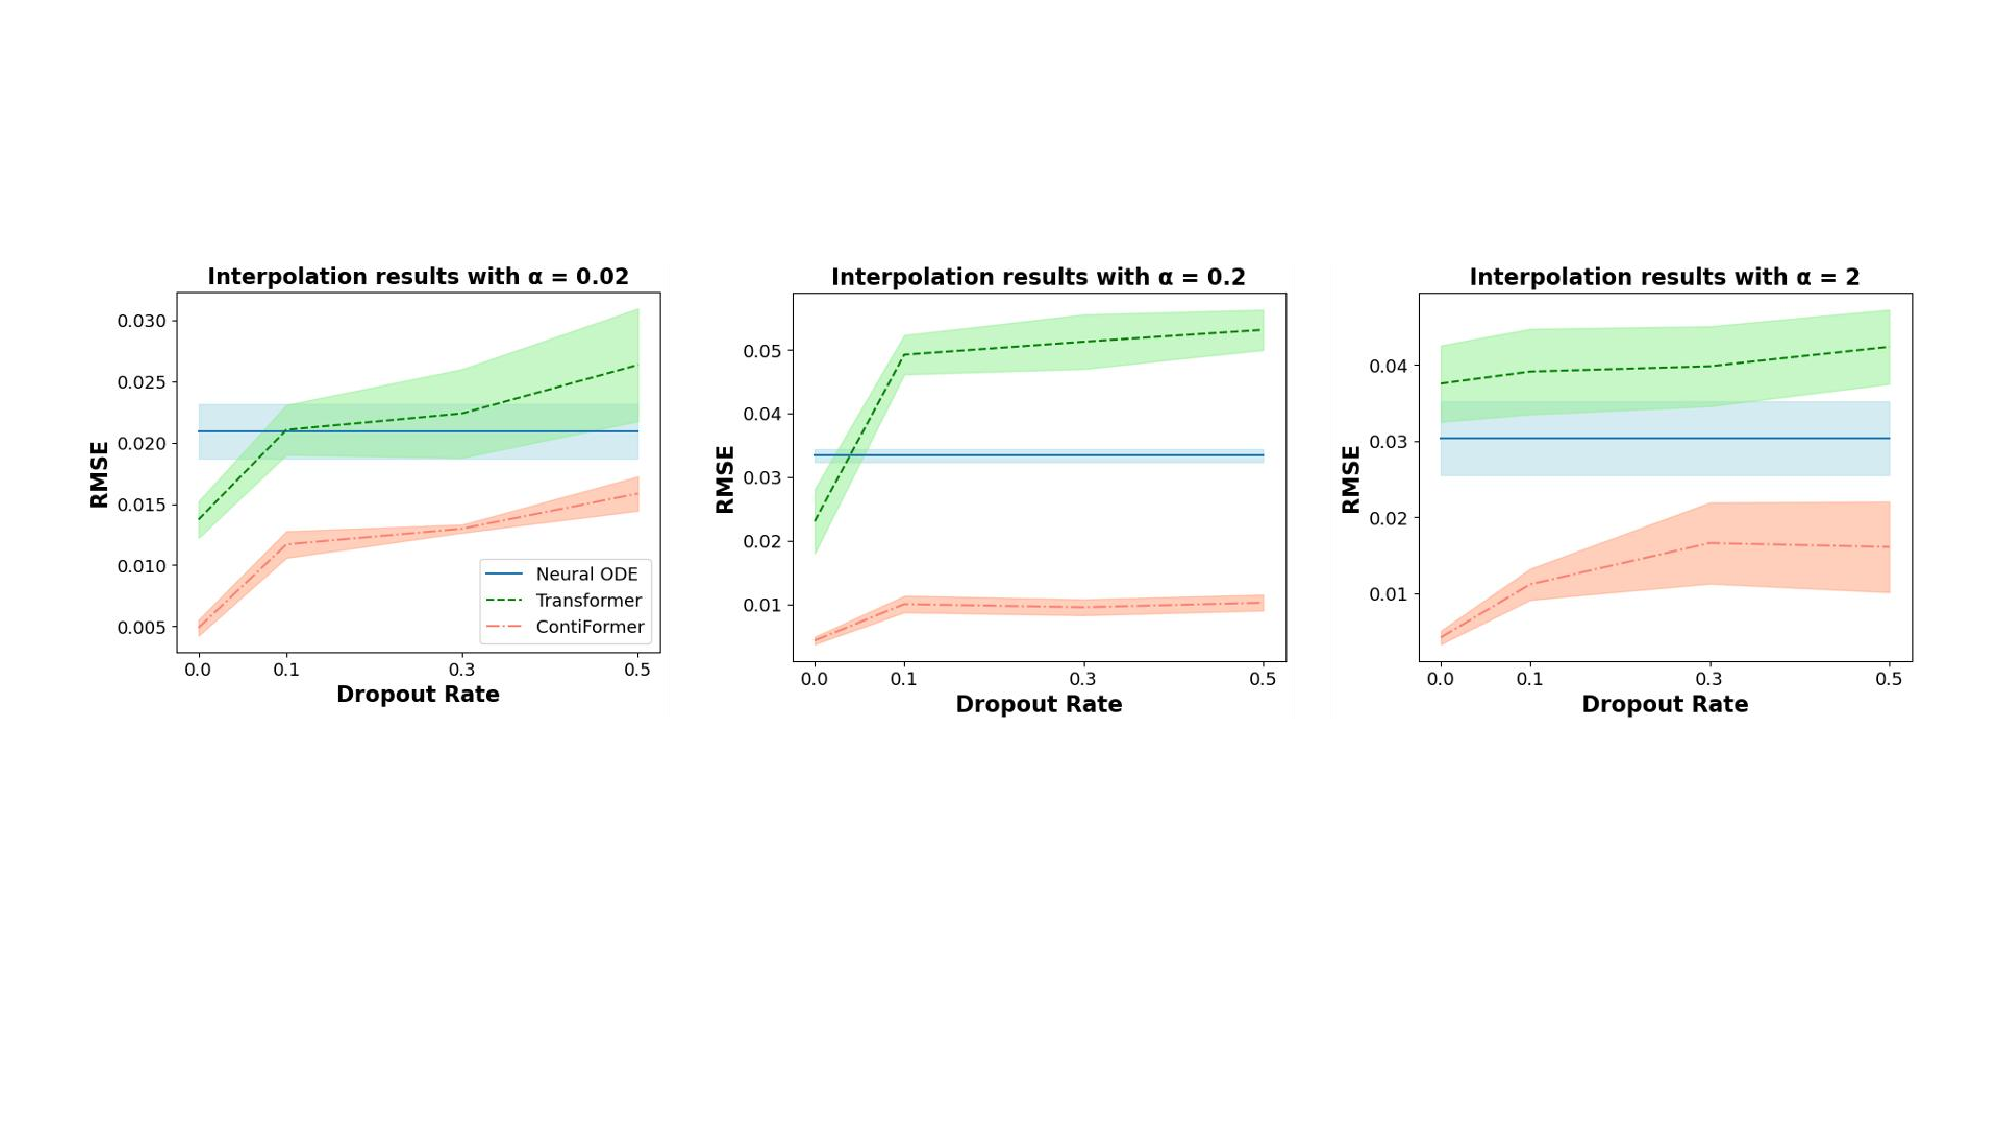
\includegraphics[width=\textwidth]{fig/dropout.pdf}
    \caption{Interpolation results on 2D spiral under different dropout rates.}
    \label{fig:dropout}
\end{figure}

Dropout in the Transformer can prevent overfitting and boost performance. However, with the increment of the dropout rate, we output of ContiFormer tends to be less continuous, leading to a sub-optimal solution for tasks that prefer a continuous-time output. To this end, we conduct experiments on both modeling continuous-time function and event prediction tasks. As for the task of modeling continuous-time function, it is desirable to have a dynamic system where outputs are ``almost'' continuous and smooth. As shown in Figure ~\ref{fig:dropout}, the performance of both Transformer and ContiFormer drops significantly as the dropout rate increases. For prediction tasks, the dynamic system can be shaky, which reflects noise or other uncontrolled influences on the system. The experimental results on event prediction can be found in Table ~\ref{tab:drp}. As shown in the table, the dropout rate has low sensitivity to the prediction results. 

\subsection{Effects of Time Normalization}

As shown in Eq. (\ref{eq:attn}) and Eq. (\ref{eq:vv}), due to the nature of sequence data, it is common to encounter abnormal points, such as events with significantly large time differences. To avoid numeric instability during training, we divide the integrated solution by the time difference. To examine the effect of normalization, we conduct experiments on 6 datasets for event prediction task. The experimental results can be found in Table ~\ref{tab:norm}, which shows that the normalization is significant on most datasets, including Synthetic, Neonate, MIMIC and StackOverflow datasets.


\begin{table*}[t]
    \centering
    \caption{Effects of dropout rate in ContiFormer on event prediction task (default to 0.1).}
    \resizebox{\textwidth}{!}{%
    \begin{tabular}{C{0.21\textwidth}C{0.07\textwidth}C{0.09\textwidth}C{0.11\textwidth}C{0.135\textwidth}C{0.135\textwidth}C{0.07\textwidth}C{0.09\textwidth}C{0.11\textwidth}}
    \toprule
         \multirow{2}{*}{\diagbox{Dropout}{Dataset}} & \multicolumn{3}{c}{Synthetic} & \multicolumn{2}{c}{Neonate} & \multicolumn{3}{c}{Traffic} \\
    \cmidrule(l){2-4}
    \cmidrule(l){5-6}
    \cmidrule(l){7-9}
          & LL ($\uparrow$) & ACC ($\uparrow$) & RMSE ($\downarrow$) & LL ($\uparrow$)  & RMSE ($\downarrow$) & LL ($\uparrow$) & ACC ($\uparrow$) & RMSE ($\downarrow$) \\
    \midrule
    0 & -0.557 & \textbf{0.842} & \textbf{0.191} & -2.588 & \textbf{9.215} & 0.633 & \textbf{0.824} & \textbf{0.328}  \\
    0.1 & \textbf{-0.535} & \textbf{0.842} & 0.192 & \textbf{-2.550} & 9.233 & \textbf{0.635} & 0.822 & \textbf{0.328} \\
    0.3 & -0.644 & \textbf{0.842} & 0.223 & -2.583 & 9.242 & 0.577 & 0.814 & 0.332 \\
    0.5 & -0.696 & 0.841 & 0.230 & -2.579 & 9.280 & 0.525 & 0.813 & 0.331 \\
    \bottomrule
    \end{tabular}}

    \resizebox{\textwidth}{!}{%
    \begin{tabular}{cccccccccc}
    \toprule
         \multirow{2}{*}{\diagbox{Dropout}{Dataset}} & \multicolumn{3}{c}{MIMIC} & \multicolumn{3}{c}{BookOrder} & \multicolumn{3}{c}{StackOverflow} \\
    \cmidrule(l){2-4}
    \cmidrule(l){5-7}
    \cmidrule(l){8-10}
          & LL ($\uparrow$) & ACC ($\uparrow$) & RMSE ($\downarrow$) &  LL ($\uparrow$) & ACC ($\uparrow$) & RMSE ($\downarrow$) & LL ($\uparrow$) & ACC ($\uparrow$) & RMSE ($\downarrow$) \\
    \midrule
    0 & -1.193 & 0.825 & 0.839 & -0.268 & 0.629 & 3.616 & -2.338 & 0.472 & 0.949 \\
    0.1 & \textbf{-1.135} & \textbf{0.836} & 0.837 & -0.270 & 0.628 & 3.614 & \textbf{-2.332} & \textbf{0.473} &\textbf{ 0.948} \\
    0.3 & -1.142 & 0.833 & \textbf{0.836} & \textbf{-0.266} & \textbf{0.630} & \textbf{3.608} & -2.336 & 0.472 & \textbf{0.948} \\
    0.5 & -1.149 & 0.834 & 0.844 & -0.270 & 0.629 & 3.624 & -2.342 & 0.471 & 0.948 \\
    \bottomrule
    \end{tabular}} 

    \label{tab:drp}
\end{table*}

\begin{table*}[t]
    \centering
    \caption{Effects of normalization on event prediction task. Attn. stands for Attention. {\scriptsize \CheckmarkBold} refers to normalizing the attention/value as shown in Eq. (\ref{eq:attn})/Eq. (\ref{eq:vv}), while {\scriptsize \XSolidBrush} refers to removing the normalization, i.e. $t - t_i$. Note that ContiFormer use both normalization for attention and values.}
    \resizebox{\textwidth}{!}{%
    \begin{tabular}{C{0.053\textwidth}C{0.053\textwidth}|C{0.07\textwidth}C{0.09\textwidth}C{0.11\textwidth}|C{0.135\textwidth}C{0.135\textwidth}|C{0.07\textwidth}C{0.09\textwidth}C{0.11\textwidth}}
    \toprule
         \multicolumn{2}{c}{Dataset} & \multicolumn{3}{c}{Synthetic} & \multicolumn{2}{c}{Neonate} & \multicolumn{3}{c}{Traffic} \\
    \cmidrule(l){1-2}
    \cmidrule(l){3-5}
    \cmidrule(l){6-7}
    \cmidrule(l){8-10}
         Attn. & Value & LL ($\uparrow$) & ACC ($\uparrow$) & RMSE ($\downarrow$) & LL ($\uparrow$)  & RMSE ($\downarrow$) & LL ($\uparrow$) & ACC ($\uparrow$) & RMSE ($\downarrow$) \\
    \midrule
    {\scriptsize \XSolidBrush} & {\scriptsize \XSolidBrush} & -0.618 & \textbf{0.842} & 0.215 & -2.612 & 9.277 & \textbf{0.721} & \textbf{0.822} & 0.329 \\
    {\scriptsize \XSolidBrush} & {\scriptsize \CheckmarkBold} & -0.601 & 0.841 & 0.206 & -2.576 & 9.240 & 0.536 & 0.814 & 0.336 \\
    {\scriptsize \CheckmarkBold} & {\scriptsize \XSolidBrush} & -0.584 & \textbf{0.842} & 0.205 & -2.601 & 9.272 & 0.576 & 0.818 & \textbf{0.327} \\
    \midrule
    {\scriptsize \CheckmarkBold} & {\scriptsize \CheckmarkBold}  & \textbf{-0.535} & \textbf{0.842} & \textbf{0.192} & \textbf{-2.550}  & \textbf{9.233} & 0.635 & \textbf{0.822} & 0.328 \\
    \bottomrule
    \end{tabular}}
    
    \resizebox{\textwidth}{!}{%
    \begin{tabular}{cc|ccc|ccc|ccc}
    \toprule
         \multicolumn{2}{c}{Dataset} & \multicolumn{3}{c}{MIMIC} & \multicolumn{3}{c}{BookOrder} & \multicolumn{3}{c}{StackOverflow} \\
    \cmidrule(l){1-2}
    \cmidrule(l){3-5}
    \cmidrule(l){6-8}
    \cmidrule(l){9-11}
         Attn. & Value & LL ($\uparrow$) & ACC ($\uparrow$) & RMSE ($\downarrow$) &  LL ($\uparrow$) & ACC ($\uparrow$) & RMSE ($\downarrow$) & LL ($\uparrow$) & ACC ($\uparrow$) & RMSE ($\downarrow$) \\
    \midrule
    {\scriptsize \XSolidBrush} & {\scriptsize \XSolidBrush} & -1.167 & 0.826 & 0.848 & -0.311 & 0.627 & 3.710 & -2.346 & 0.470 & \textbf{0.948} \\
    {\scriptsize \XSolidBrush} & {\scriptsize \CheckmarkBold} & -1.149 & 0.833 & 0.840 & \textbf{-0.269} & \textbf{0.630} & 3.634 & -2.341 & 0.471 & \textbf{0.948} \\
    {\scriptsize \CheckmarkBold} & {\scriptsize \XSolidBrush} & -1.172 & 0.826 & 0.844 & -0.277 & 0.629 & 3.654 & -2.336 & \textbf{0.472} & \textbf{0.948} \\
    \midrule
    {\scriptsize \CheckmarkBold} & {\scriptsize \CheckmarkBold} & \textbf{-1.135} & \textbf{0.836} & \textbf{0.837} & -0.270 & 0.628 & \textbf{3.614} & \textbf{-2.334} & \textbf{0.472} & \textbf{0.948} \\
    \bottomrule
    \end{tabular}}
    
    \label{tab:norm}
\end{table*}

\section{Time Cost v.s. Memory Cost v.s. Accuracy} \label{sec:cost}

\begin{table}[t]
    \centering
    \caption{Time Cost v.s. Accuracy for different models on UEA classification datasets (0\% dropped). For all ODE-based models and our model, we adopt the RK4 solver and step size refers to the amount of time increment for the RK4 solver. $\uparrow$ ($\downarrow$) indicates the higher (lower) the better. Note that since the results are aggregated over 3 random seeds, achieving the same results doesn't indicate the same outcome for each random seed.}
    \resizebox{\textwidth}{!}{%
    \begin{tabular}{cccccccc}
    \toprule
        Dataset & & \multicolumn{2}{c}{BasicMotions} & \multicolumn{2}{c}{JapaneseVowels} &  \multicolumn{2}{c}{Libras}  \\ 
        Model & Step Size & Time Cost ($\downarrow$) & Accuracy ($\uparrow$) &  Time Cost ($\downarrow$) & Accuracy ($\uparrow$) & Time Cost ($\downarrow$) & Accuracy ($\uparrow$)  \\ 
    \midrule
        TST & - & $0.56 \times$  & 0.975  & $0.10 \times$  & 0.986  & $0.36 \times$  & 0.843  \\ 
        S5 & - & $1 \times$  & 0.958  & $1 \times$  & 0.926  & $1 \times$  & 0.655  \\ 
    \midrule
        \multirow{2}{*}{ODE-RNN (w/o norm)} & 0.1 & $3.06 \times$  & 0.917  & $0.79 \times$  & 0.952  & $2.67 \times$  & 0.602  \\ 
        ~ & 0.01 & $18.94 \times$  & 0.925  & $5.26 \times$  & 0.955  & $16.29 \times$  & 0.611  \\ 
    \midrule
        \multirow{2}{*}{ODE-RNN (w/ norm)} & 0.1 & $1.46 \times$  & \textbf{1.000}  & $0.32 \times$  & 0.980  & $1.24 \times$  & 0.637  \\ 
        ~ & 0.01 & $1.59 \times$  & \textbf{1.000}  & $0.47 \times$  & 0.980  & $1.59 \times$  & 0.619  \\ 
    \midrule
        \multirow{2}{*}{Neural CDE} & 0.1 & $4.47 \times$  & 0.958  & $1.16 \times$  & 0.932  & $3.87 \times$  & 0.763  \\ 
        ~ & 0.01 & $34.26 \times$  & 0.958  & $9.57 \times$  & 0.942  & $28.48 \times$  & 0.744  \\ 
    \midrule
        \multirow{2}{*}{ContiFormer} & 0.1 & $2.89 \times$  & 0.975  & $0.49 \times$  & 0.990  & $2.26 \times$  & \textbf{0.870}  \\ 
        ~ & 0.01 & $13.75 \times$  & 0.975  & $1.87 \times$  & \textbf{0.991}  & $8.74 \times$  & \textbf{0.870} \\ 
    \bottomrule
    \end{tabular}}

    \resizebox{\textwidth}{!}{%
    \begin{tabular}{cccccccc}
    \toprule
        Dataset & & \multicolumn{2}{c}{NATOPS} & \multicolumn{2}{c}{PEMS-SF} &  \multicolumn{2}{c}{RacketSports}  \\ 
        Model & Step Size & Time Cost ($\downarrow$) & Accuracy ($\uparrow$) &  Time Cost ($\downarrow$) & Accuracy ($\uparrow$) & Time Cost ($\downarrow$) & Accuracy ($\uparrow$)  \\ 
    \midrule
        TST & - & $0.32 \times$  & \textbf{0.963}  & $0.15 \times$  & 0.890  & $0.14 \times$ & 0.826  \\ 
        S5 & - & $1 \times$  & 0.839  & $1 \times$  & \textbf{0.896}  & $1 \times$  & 0.772  \\ 
    \midrule
        \multirow{2}{*}{ODE-RNN (w/o norm)} & 0.1 & $2.67 \times$  & 0.909  & $4 \times$  & 0.778  & $2.47 \times$  & 0.827  \\ 
        ~ & 0.01 & $16.52 \times$  & 0.907  & $28.45 \times$  & 0.761  & $14.65 \times$  & 0.796  \\ 
    \midrule
        \multirow{2}{*}{ODE-RNN (w/ norm)} & 0.1 & $1.28 \times$  & 0.898  & $1.47 \times$  & 0.775  & $1.15 \times$  & 0.785  \\ 
        ~ & 0.01 & $1.45 \times$  & 0.898  & $1.44 \times$  & 0.775  & $1.57 \times$  & 0.787  \\ 
    \midrule
        \multirow{2}{*}{Neural CDE} & 0.1 & $3.83 \times$  & 0.789  & $6.04 \times$  & 0.763  & $3.48 \times$  & 0.743  \\ 
        ~ & 0.01 & $29.24 \times$ & 0.787  & $50.36 \times$  & 0.763  & $25.04 \times$  & 0.748  \\ 
    \midrule
        \multirow{2}{*}{ContiFormer} & 0.1 & $2.32 \times$  & 0.935  & $5.45 \times$  & 0.823  & $1.87 \times$  & \textbf{0.836}  \\ 
        ~ & 0.01 & $9.76 \times$  & 0.935  & $37.08 \times$  & 0.823  & $5.88 \times$  & \textbf{0.836} \\ 
    \bottomrule
    \end{tabular}}
    
    \label{tab:costfull}
\end{table}

\begin{figure}[htbp]
    \centering
    \vspace{20pt}
    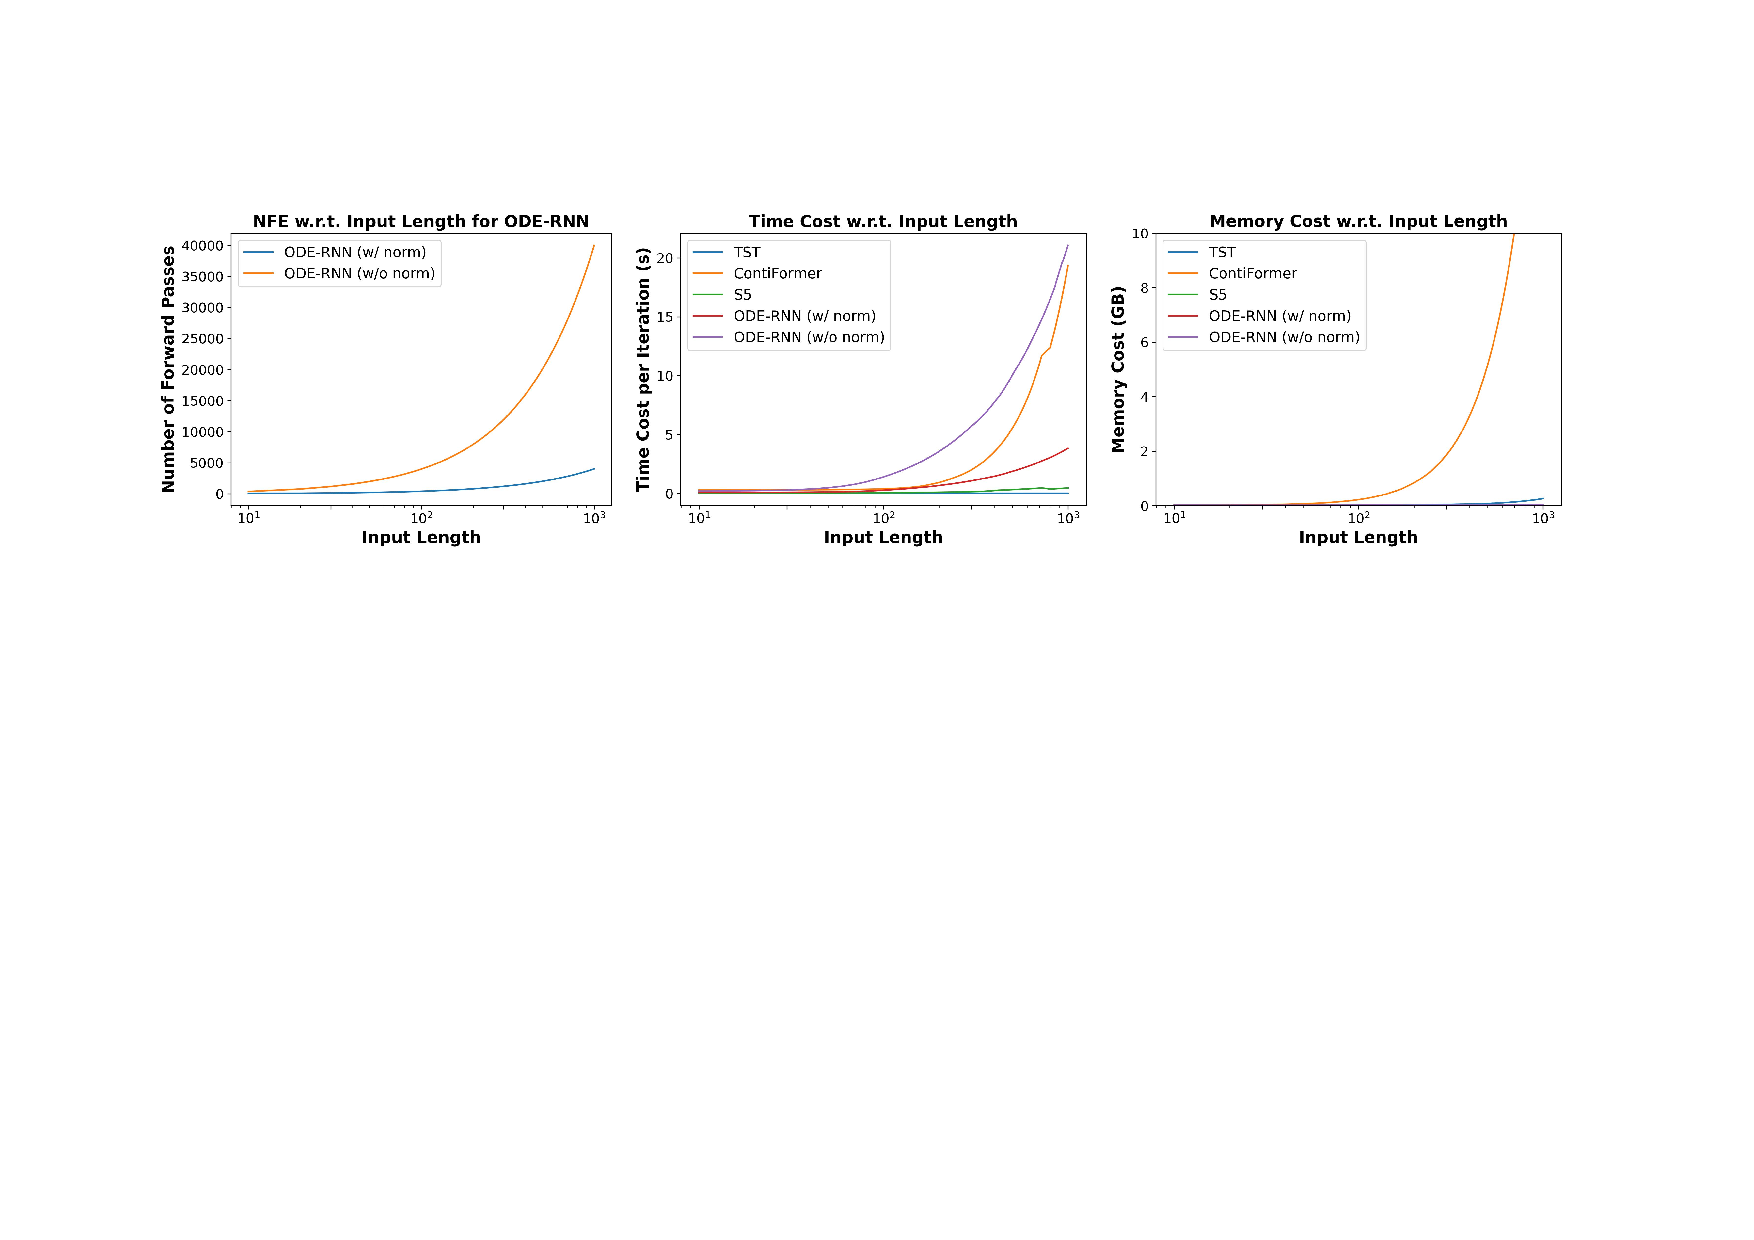
\includegraphics[width=\textwidth]{fig/cost.pdf}
    \caption{Time Cost v.s. Memory Cost v.s. Accuracy.}
    \label{fig:cost}
\end{figure}


Utilizing continuous-time modeling in ContiFormer often results in substantial time and GPU memory overhead. We have conducted a comparative analysis of ContiFormer's actual time costs in comparison to Transformer-based models (TST), ODE-based models (ODE-RNN, Neural CDE), and SSM-based models (S5). Throughout our analysis, we employ an RK4 solver for ODE-based models and our model, setting the step size to $0.1$ and $0.01$. It's worth noting that, for ODE-RNN and other ODE-based models, the input times have an impact on the number of forward passes when using a fixed-step ODE solver, thus, affecting the time costs.

The left figure in Figure \ref{fig:cost} illustrates the influence of input times concerning input length. For the model with normalization (a.k.a., w/ norm), the input times consistently range from $[0,1]$, regardless of the input length. Conversely, for the model without normalization (a.k.a., w/o norm), the input times span from $[0, L]$, where $L$ represents the input length.

As depicted in the middle figure in Figure \ref{fig:cost}, our model performs comparably to ODE-RNN (w/ norm) when the input length is up to $100$, but becomes approximately four times slower as the input length extends to $1000$. The right figure in Figure \ref{fig:cost} displays GPU memory usage, revealing a significantly higher memory cost associated with our model.

Table \ref{tab:costfull} provides a more comprehensive overview of different models on UEA datasets. It is evident that our model strikes a better balance between accuracy and time cost. Specifically, our model achieves the best performance on 3 out of 6 selected datasets while incurring only twice the time cost compared to S5.

\newpage
\section{Broader Impact}

The proposed model, ContiFormer, presents several potential impacts within the field of machine learning and irregular time series analysis. These include:
\begin{itemize}[leftmargin=5mm]
    \item Enhanced Modeling Capability: ContiFormer extends the Transformer architecture to effectively capture complex continuous-time dynamic systems. By leveraging continuous-time modeling techniques, the model demonstrates improved performance in handling irregular time series data, offering a more flexible and powerful modeling ability.
    \item Practical Applications: Our proposed method achieves state-of-the-art performance in a variety of tasks and real-life datasets, which makes it more promising to tackle real-world applications. The ability to model continuous-time dynamics offers valuable insights into time-evolving systems, facilitating improved decision-making and predictive capabilities in diverse domains.
\end{itemize}